% Options for packages loaded elsewhere
\PassOptionsToPackage{unicode}{hyperref}
\PassOptionsToPackage{hyphens}{url}
\PassOptionsToPackage{dvipsnames,svgnames,x11names}{xcolor}
%
\documentclass[
  letterpaper,
  DIV=11,
  numbers=noendperiod]{scrreprt}

\usepackage{amsmath,amssymb}
\usepackage{iftex}
\ifPDFTeX
  \usepackage[T1]{fontenc}
  \usepackage[utf8]{inputenc}
  \usepackage{textcomp} % provide euro and other symbols
\else % if luatex or xetex
  \usepackage{unicode-math}
  \defaultfontfeatures{Scale=MatchLowercase}
  \defaultfontfeatures[\rmfamily]{Ligatures=TeX,Scale=1}
\fi
\usepackage{lmodern}
\ifPDFTeX\else  
    % xetex/luatex font selection
\fi
% Use upquote if available, for straight quotes in verbatim environments
\IfFileExists{upquote.sty}{\usepackage{upquote}}{}
\IfFileExists{microtype.sty}{% use microtype if available
  \usepackage[]{microtype}
  \UseMicrotypeSet[protrusion]{basicmath} % disable protrusion for tt fonts
}{}
\makeatletter
\@ifundefined{KOMAClassName}{% if non-KOMA class
  \IfFileExists{parskip.sty}{%
    \usepackage{parskip}
  }{% else
    \setlength{\parindent}{0pt}
    \setlength{\parskip}{6pt plus 2pt minus 1pt}}
}{% if KOMA class
  \KOMAoptions{parskip=half}}
\makeatother
\usepackage{xcolor}
\setlength{\emergencystretch}{3em} % prevent overfull lines
\setcounter{secnumdepth}{5}
% Make \paragraph and \subparagraph free-standing
\ifx\paragraph\undefined\else
  \let\oldparagraph\paragraph
  \renewcommand{\paragraph}[1]{\oldparagraph{#1}\mbox{}}
\fi
\ifx\subparagraph\undefined\else
  \let\oldsubparagraph\subparagraph
  \renewcommand{\subparagraph}[1]{\oldsubparagraph{#1}\mbox{}}
\fi

\usepackage{color}
\usepackage{fancyvrb}
\newcommand{\VerbBar}{|}
\newcommand{\VERB}{\Verb[commandchars=\\\{\}]}
\DefineVerbatimEnvironment{Highlighting}{Verbatim}{commandchars=\\\{\}}
% Add ',fontsize=\small' for more characters per line
\usepackage{framed}
\definecolor{shadecolor}{RGB}{241,243,245}
\newenvironment{Shaded}{\begin{snugshade}}{\end{snugshade}}
\newcommand{\AlertTok}[1]{\textcolor[rgb]{0.68,0.00,0.00}{#1}}
\newcommand{\AnnotationTok}[1]{\textcolor[rgb]{0.37,0.37,0.37}{#1}}
\newcommand{\AttributeTok}[1]{\textcolor[rgb]{0.40,0.45,0.13}{#1}}
\newcommand{\BaseNTok}[1]{\textcolor[rgb]{0.68,0.00,0.00}{#1}}
\newcommand{\BuiltInTok}[1]{\textcolor[rgb]{0.00,0.23,0.31}{#1}}
\newcommand{\CharTok}[1]{\textcolor[rgb]{0.13,0.47,0.30}{#1}}
\newcommand{\CommentTok}[1]{\textcolor[rgb]{0.37,0.37,0.37}{#1}}
\newcommand{\CommentVarTok}[1]{\textcolor[rgb]{0.37,0.37,0.37}{\textit{#1}}}
\newcommand{\ConstantTok}[1]{\textcolor[rgb]{0.56,0.35,0.01}{#1}}
\newcommand{\ControlFlowTok}[1]{\textcolor[rgb]{0.00,0.23,0.31}{#1}}
\newcommand{\DataTypeTok}[1]{\textcolor[rgb]{0.68,0.00,0.00}{#1}}
\newcommand{\DecValTok}[1]{\textcolor[rgb]{0.68,0.00,0.00}{#1}}
\newcommand{\DocumentationTok}[1]{\textcolor[rgb]{0.37,0.37,0.37}{\textit{#1}}}
\newcommand{\ErrorTok}[1]{\textcolor[rgb]{0.68,0.00,0.00}{#1}}
\newcommand{\ExtensionTok}[1]{\textcolor[rgb]{0.00,0.23,0.31}{#1}}
\newcommand{\FloatTok}[1]{\textcolor[rgb]{0.68,0.00,0.00}{#1}}
\newcommand{\FunctionTok}[1]{\textcolor[rgb]{0.28,0.35,0.67}{#1}}
\newcommand{\ImportTok}[1]{\textcolor[rgb]{0.00,0.46,0.62}{#1}}
\newcommand{\InformationTok}[1]{\textcolor[rgb]{0.37,0.37,0.37}{#1}}
\newcommand{\KeywordTok}[1]{\textcolor[rgb]{0.00,0.23,0.31}{#1}}
\newcommand{\NormalTok}[1]{\textcolor[rgb]{0.00,0.23,0.31}{#1}}
\newcommand{\OperatorTok}[1]{\textcolor[rgb]{0.37,0.37,0.37}{#1}}
\newcommand{\OtherTok}[1]{\textcolor[rgb]{0.00,0.23,0.31}{#1}}
\newcommand{\PreprocessorTok}[1]{\textcolor[rgb]{0.68,0.00,0.00}{#1}}
\newcommand{\RegionMarkerTok}[1]{\textcolor[rgb]{0.00,0.23,0.31}{#1}}
\newcommand{\SpecialCharTok}[1]{\textcolor[rgb]{0.37,0.37,0.37}{#1}}
\newcommand{\SpecialStringTok}[1]{\textcolor[rgb]{0.13,0.47,0.30}{#1}}
\newcommand{\StringTok}[1]{\textcolor[rgb]{0.13,0.47,0.30}{#1}}
\newcommand{\VariableTok}[1]{\textcolor[rgb]{0.07,0.07,0.07}{#1}}
\newcommand{\VerbatimStringTok}[1]{\textcolor[rgb]{0.13,0.47,0.30}{#1}}
\newcommand{\WarningTok}[1]{\textcolor[rgb]{0.37,0.37,0.37}{\textit{#1}}}

\providecommand{\tightlist}{%
  \setlength{\itemsep}{0pt}\setlength{\parskip}{0pt}}\usepackage{longtable,booktabs,array}
\usepackage{calc} % for calculating minipage widths
% Correct order of tables after \paragraph or \subparagraph
\usepackage{etoolbox}
\makeatletter
\patchcmd\longtable{\par}{\if@noskipsec\mbox{}\fi\par}{}{}
\makeatother
% Allow footnotes in longtable head/foot
\IfFileExists{footnotehyper.sty}{\usepackage{footnotehyper}}{\usepackage{footnote}}
\makesavenoteenv{longtable}
\usepackage{graphicx}
\makeatletter
\def\maxwidth{\ifdim\Gin@nat@width>\linewidth\linewidth\else\Gin@nat@width\fi}
\def\maxheight{\ifdim\Gin@nat@height>\textheight\textheight\else\Gin@nat@height\fi}
\makeatother
% Scale images if necessary, so that they will not overflow the page
% margins by default, and it is still possible to overwrite the defaults
% using explicit options in \includegraphics[width, height, ...]{}
\setkeys{Gin}{width=\maxwidth,height=\maxheight,keepaspectratio}
% Set default figure placement to htbp
\makeatletter
\def\fps@figure{htbp}
\makeatother

\KOMAoption{captions}{tableheading}
\makeatletter
\makeatother
\makeatletter
\@ifpackageloaded{bookmark}{}{\usepackage{bookmark}}
\makeatother
\makeatletter
\@ifpackageloaded{caption}{}{\usepackage{caption}}
\AtBeginDocument{%
\ifdefined\contentsname
  \renewcommand*\contentsname{Table of contents}
\else
  \newcommand\contentsname{Table of contents}
\fi
\ifdefined\listfigurename
  \renewcommand*\listfigurename{List of Figures}
\else
  \newcommand\listfigurename{List of Figures}
\fi
\ifdefined\listtablename
  \renewcommand*\listtablename{List of Tables}
\else
  \newcommand\listtablename{List of Tables}
\fi
\ifdefined\figurename
  \renewcommand*\figurename{Figure}
\else
  \newcommand\figurename{Figure}
\fi
\ifdefined\tablename
  \renewcommand*\tablename{Table}
\else
  \newcommand\tablename{Table}
\fi
}
\@ifpackageloaded{float}{}{\usepackage{float}}
\floatstyle{ruled}
\@ifundefined{c@chapter}{\newfloat{codelisting}{h}{lop}}{\newfloat{codelisting}{h}{lop}[chapter]}
\floatname{codelisting}{Listing}
\newcommand*\listoflistings{\listof{codelisting}{List of Listings}}
\makeatother
\makeatletter
\@ifpackageloaded{caption}{}{\usepackage{caption}}
\@ifpackageloaded{subcaption}{}{\usepackage{subcaption}}
\makeatother
\makeatletter
\@ifpackageloaded{tcolorbox}{}{\usepackage[skins,breakable]{tcolorbox}}
\makeatother
\makeatletter
\@ifundefined{shadecolor}{\definecolor{shadecolor}{rgb}{.97, .97, .97}}
\makeatother
\makeatletter
\makeatother
\makeatletter
\makeatother
\ifLuaTeX
  \usepackage{selnolig}  % disable illegal ligatures
\fi
\IfFileExists{bookmark.sty}{\usepackage{bookmark}}{\usepackage{hyperref}}
\IfFileExists{xurl.sty}{\usepackage{xurl}}{} % add URL line breaks if available
\urlstyle{same} % disable monospaced font for URLs
\hypersetup{
  pdftitle={EDUC 784},
  pdfauthor={Peter Halpin},
  colorlinks=true,
  linkcolor={blue},
  filecolor={Maroon},
  citecolor={Blue},
  urlcolor={Blue},
  pdfcreator={LaTeX via pandoc}}

\title{EDUC 784}
\author{Peter Halpin}
\date{2024-01-03}

\begin{document}
\maketitle
\ifdefined\Shaded\renewenvironment{Shaded}{\begin{tcolorbox}[frame hidden, borderline west={3pt}{0pt}{shadecolor}, boxrule=0pt, enhanced, breakable, interior hidden, sharp corners]}{\end{tcolorbox}}\fi

\renewcommand*\contentsname{Table of contents}
{
\hypersetup{linkcolor=}
\setcounter{tocdepth}{2}
\tableofcontents
}
\bookmarksetup{startatroot}

\hypertarget{preface}{%
\chapter*{Preface}\label{preface}}
\addcontentsline{toc}{chapter}{Preface}

\markboth{Preface}{Preface}

These are the course notes for EDUC 784. Readings are assigned
\emph{before class.} Sections denoted with an asterisk (*) are optional.

The notes contain \textbf{questions that are written in bold font}. The
questions are also collected in a section called ``Workbook'' that
appears towards the end of each chapter. During class time, we will
discuss the Workbook questions, your answers, any additional question
you have, etc. It is really important for you to do the readings, and
write down your responses to the questions, before class. You won't get
much out of the lessons if you haven't done this preparation.

Some chapters contain a section called ``Exercises'' that collects all
of the R code from that chapter into a single overall workflow.
\textbf{You don't need to do the Exercises before class}, but you can if
you want to. If a chapter doesn't have an Exercises section, that means
we will be working on an assignment together instead.

\bookmarksetup{startatroot}

\hypertarget{sec-chap-1}{%
\chapter{Review}\label{sec-chap-1}}

This chapter is an exception to the overall format described in the
Preface. It reviews some foundational material from EDUC 710 (Stat 1)
that is useful for this course. There will be time to ask questions
about the review material in the first class and second class, but there
will not be time to review everything. So, if this review feels too
short, you may also want to review your notes from EDUC 710.

Please review up to the Exercises in Section~\ref{sec-exercizes-1}
before the first class. We will address any questions about this
material in the first class and then begin the Exercises together.

\hypertarget{sec-summation-1}{%
\section{Summation notation}\label{sec-summation-1}}

Summation notation uses the symbol \(\Sigma\) to stand-in for summation.
For example, instead of writing

\[ X_1 + X_2 + X_3 + .... + X_N\]

to represent the sum of the values of the variable \(X\) in a sample of
size \(N\), we can instead write:

\[ \sum_{i=1}^{N} X_i. \]

The symbol \(\Sigma\) means ``add.'' The symbol is called ``Sigma'' --
it's the capital Greek letter corresponding to the Latin letter ``S''.
The value \(i\) is called the index, and \(1\) is the starting value of
the index and \(N\) is the end value of the index. You can choose
whatever start and end values you want to sum over. For example, if we
just want to add the second and third values of \(X\), we write

\[ \sum_{i=2}^{3} X_i = X_2 + X_3. \]

When the start and end evalues are clear from context, we can use a
shorthand notation that omits them. In the following, it is implicit
that the sum is over the all available values of \(X\) (i.e., from \(1\)
to \(N\)):

\[ \sum_i X_i. \]

\hypertarget{sec-rules-1}{%
\section{Rules of summation}\label{sec-rules-1}}

There are rules for manipulating summation notation that are useful for
deriving results in statistics. These rules are things you learned about
addition in grade school, but they are presented using summation
notation. You don't need to do mathematical proofs or derivations in
this class, but you will occasionally see some derivations in these
notes (mainly in the optional sections).

Here are the rules:

\textbf{Rule 1: Sum of a constant (multiplication)}. Summing the values
of a constant \(c\) is the same as multiplication. Specifically, if you
add a constant \(c\) to itself \(N\) times, this just \(N\) times the
constant:

\begin{align}
\sum_{i = 1}^{N} c &= c + c +  .... \\
& = Nc 
\end{align}

\textbf{Rule 2: Distributive property}. The sum of a variable \(X_i\)
times a constant \(c\) is equal to the constant times the sum.

\begin{align}
\sum_{i = 1}^{N} c X_i &= cX_1 + cX_2 + .... \\
& = c(X_1 + X_2 + ....) \\ 
& = c \sum_{i = 1}^{N} X_i 
\end{align}

\textbf{Rule 3: Associative property}. It doesn't matter what order we
do addition in:

\begin{align}
\sum_{i = 1}^{N} (X_i + Y_i) &= (X_1 + Y_1) + (X_2 + Y_2) + .... \\
& = (X_1 + X_2 + ....) + (Y_1 + Y_2 + ....) \\
& = \sum_{i = 1}^{N} X_i  + \sum_{i = 1}^{N} Y_i 
\end{align}

\hypertarget{sec-stats-1}{%
\section{Sample statistics}\label{sec-stats-1}}

Summation notation is useful for writing the formulas of statistics. The
main statistics we use in the class are the mean, standard deviation,
variance, covariance, and correlation. These are the building blocks for
regression. Their symbols and formulas are presented below (using the
shorthand summation notation). If you don't remember their
interpretation, you will need to go back to your Stat 1 notes.

\begin{itemize}
\tightlist
\item
  The mean
\end{itemize}

\[\bar X = \frac{\sum_i X_i}{N}\]

\begin{itemize}
\tightlist
\item
  The variance can be written as \(\text{var}(X)\) or sometimes using
  the symbol \(s^2\)
\end{itemize}

\[ \text{var}(X) = \frac{\sum_i (X_i - \bar X)^2}{N - 1} \]

\begin{itemize}
\tightlist
\item
  The standard deviation can be written \(\text{SD}(X)\) or using the
  letter \(s\)
\end{itemize}

\[ \text{SD}(X) = \sqrt{\text{var}(X)} \]

\begin{itemize}
\tightlist
\item
  The covariance is a generalization of the variance to two variables,
  it describes how they co-vary:
\end{itemize}

\[\text{cov}(X, Y) = \frac{\sum_i (X_i - \bar X) (Y_i - \bar Y)}{N - 1} \]

\begin{itemize}
\tightlist
\item
  The correlation is the covariance divided by the product of the
  standard deviations of the variables. It takes on values between -1
  and 1 and describes the strength and direction of the linear
  relationship between two variables.
\end{itemize}

\[\text{cor}(X, Y) = \frac{\text{cov}(X, Y)}{\sqrt{\text{var}(X)} \sqrt{\text{var}(Y)}} \]

For numerical examples see Section~\ref{sec-computing-stats-1}.

\hypertarget{sec-properties-1}{%
\section{Some properties of sample statistics}\label{sec-properties-1}}

The following are some useful properties of the sample statistics
reviewed above. You can derive these properties using the rules of
summation. For each property, the beginning of the derivation is shown.
You should know the properties but completing the derivations is
optional.

\textbf{Sum of deviations from the mean}. If we subtract the mean from
each data point, we have what is called a deviation (or deviation
score): \(d_i = X_i - \bar X\). It is always the case that
\(\sum_i d_i = 0\)

\begin{itemize}
\tightlist
\item
  Derivation
\end{itemize}

\[ \sum_i d_i = \sum_i(X_i - \bar X) = \dots \]

\textbf{Mean of a linear transformation}. If \(Y_i = A + B X_i\) with
known constants \(A\) and \(B\), then \(\bar{Y} = A + B \bar{X}\)

\begin{itemize}
\tightlist
\item
  Derivation:
\end{itemize}

\[ \bar{Y} =  \frac{\sum_i Y_i}{N} =  \frac{\sum_i( A + B X_i)}{N} = \dots \]
\textbf{Variance of a linear transformation}. If \(Y_i = A + B X_i\)
with known constants \(A\) and \(B\), then
\(\text{var}(Y) = B^2\text{var}(X)\)

\begin{itemize}
\tightlist
\item
  Derivation
\end{itemize}

\[ \text{var}(Y) =  \frac{\sum_i (Y_i - \bar{Y})^2}{N-1} =  \frac{\sum_i ((A + B X_i) - (A + B \bar{X}))^2}{N-1} = \dots\]
\textbf{Mean and variance of a z-score}. The z-score (or standardized
score) is defined as \(Z_i = (X_i - \bar{X}) / \text{SD}(X)\).
Standardized scores are useful because they have \(\bar{Z} = 0\) and
\(\text{var}(Z) = 1\).

\begin{itemize}
\tightlist
\item
  Derivation: use the rules for linear transformation with
  \(A = -\bar{X} / \text{SD}(X)\) and \(B = 1/ \text{SD}(X)\).
\end{itemize}

\textbf{Covariance of linear transformation}. If \(Y_i = A + B X_i\) and
\(W_i = C + D U_i\) with known constants \(A\), \(B\), \(C\), \(D\),
then \(\text{cov}(Y, W) = BD\,\text{cov}(X, U)\)

\begin{itemize}
\tightlist
\item
  Derivation
\end{itemize}

\[ \text{cov}(Y, W) =  \frac{\sum_i ((A + B X_i) - (A + B \bar{X}))((C + D U_i) - (C + D \bar{U}))}{N-1} = \dots\]

\textbf{Correlation of linear transformation}. If \(Y_i = A + B X_i\)
and \(W_i = C + D U_i\) with known constants \(A\), \(B\), \(C\), \(D\),
then \(\text{cor}(Y, W) = \text{cor}(X, U)\) -- i.e., the correlation is
not affected by linear transformations.

\begin{itemize}
\tightlist
\item
  Derivation: use the rules for variances and covariances of linear
  transformation and the formula for correlation.
\end{itemize}

\hypertarget{bias-and-precision}{%
\section{Bias and precision}\label{bias-and-precision}}

In this section we consider two more important properties of a
statistic. These properties are defined in terms of the \emph{sampling
distribution} of a statistic. Recall that a sampling distribution arise
from the following thought experiment: 1. Take a random sample of size
\(N\) from a population of interest. 2. Compute a statistic using the
sample data. It can be any statistic, but let's say the mean,
\(\bar X\), for concreteness. 3. Write down the value of the mean, and
then return the sample to the population.

After doing these 3 steps many times, you will have many values the
sample mean,

\[ \bar{X}_1, \bar{X}_2, \bar{X}_3, \bar{X}_4, \bar{X}_5 ... \]

The distribution of these sample means is called the sampling
distribution (of the mean).

A sampling distribution is just like any other distribution -- so it has
its own mean, and its own variance, etc. These statistics, when computed
for a sampling distribution, have special names. We are espeically
interested in the following two statistics.

\begin{itemize}
\item
  \textbf{The expected value} of the mean, denoted \(E(\bar X)\), is the
  mean of the sampling distribution of the mean. That is a mouthful!
  That is why we say the expected value of a statistic rather than the
  mean of a statistic. It's called the expected value because it's the
  average value over many samples.
\item
  \textbf{The standard error} of the mean, denoted \(SE(\bar X)\), is
  the standard deviation of the sampling distribution of the mean. It
  describes the sample-to-sample variation of the mean around its
  expected value.
\end{itemize}

Now for the two additional properties of a statistic:

\begin{itemize}
\item
  \textbf{Bias}: If the expected value of a statistic is equal to a
  population parameter, we say that the statistic is an unbiased
  estimate of that parameter. For example, the expected value of the
  sample mean is equal to the population mean (in symbols:
  \(E(\bar{X}) = \mu)\), so we say that the sample mean is an unbiased
  estimate of the population mean.
\item
  \textbf{Precision}: The inverse of the squared standard error (i.e.,
  \(1 / \text{SE}(\bar{X})^2\)) is called the precision of a statistic.
  So, the less a statistic varies from sample to sample, the more
  precise it is. That should hopefully make intuitive sense. The main
  thing to know about precision is that it is usually increasing in the
  sample size -- i.e., we get more precise estimates by using larger
  samples. Again, this should feel intuitive.
\end{itemize}

Below is a figure that is often used to illustrate the ideas of bias and
precision. The middle of the concentric circles represent the target
parameter (like a bull's eye) and the dots represent the sampling
distribution of a statistic. You should be able to describe each panel
in terms of the bias and precision of the statistic.

\begin{figure}

{\centering 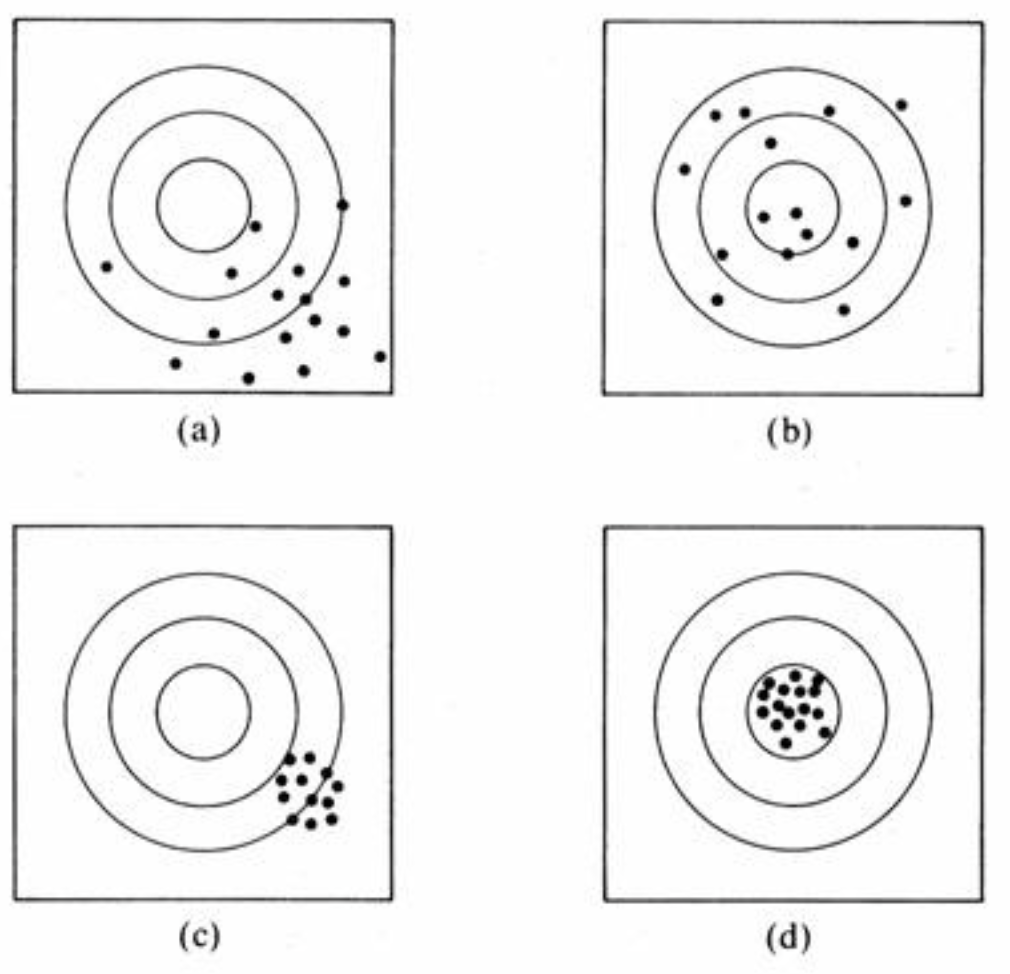
\includegraphics[width=4.16667in,height=\textheight]{files/images/bias_and_precision.png}

}

\caption{\label{fig-bnp}Bias and Precision}

\end{figure}

\hypertarget{t-tests}{%
\section{t-tests}\label{t-tests}}

The \(t\)-test is used to make an inference about the value of an
unknown population parameter. The test compares the value of an unbiased
estimate of the parameter to a hypothesized value of the parameter. The
conceptual formula for a \(t\)-test is

\[ t = \frac{\text{unbiased estimate} - \text{hypothesized value }}{\text{standard error}} \]

When we conduct a \(t\)-test, the basic rationale is as follows: ``if
the estimate statistic is close the hypothesized value of the parameter,
then the numerator should be small relative to the standard error, and
so \(t\) should be close to zero.''

Typically, the hypothesized value of the population parameter is equal
to zero, in which case it is called a null hypothesis. The null
hypothesis usually translates into a research hypothesis of ``no
effect'' or ``no relationship.'' So, if \(t\) is close to zero, it means
there was no effect.

In order to determine what values of \(t\) are ``close to zero'', we
refer to its sampling distribution, which is called the
\(t\)-distribution. The \(t\)-distribution tells what values of \(t\)
are typical if the null hypothesis is true. (More specifically: if the
sample statistic is normally distributed and its expected value equal to
the hypothesized value, then \(t\) has a ``central''
\(t\)-distribution.)

Some examples of the \(t\)-distribution are shown below. The x-axis
denotes values of the statistic \(t\) shown above, and \(\nu\) is a
parameter called the ``degrees of freedom'' (more on this below). You
can see that the \(t\)-distribution looks like a normal distribution
centered a zero. So, when the null hypothesis is true, the expected
value of \(t\) is zero. Informally, we could say that values greater
than \(\pm 2\) are pretty unlikely, and values greater than \(\pm 4\)
are very unlikely. Keep in the mind that these are the values of \(t\)
we are expecting if the null hypothesis is true.

\begin{figure}

{\centering \includegraphics[width=4.16667in,height=\textheight]{index_files/mediabag/1920px-Student_t_pdf.png}

}

\caption{\label{fig-tdist}t-distribution (source:
https://en.wikipedia.org/wiki/Student\%27s\_t-distribution)}

\end{figure}

More formally, we can compare the value of \(t\) computed in a sample,
denoted as \(t_{\text{obs}}\), to a ``critical value'', denoted as
\(t^*\). The critical value is chosen so that the ``significance
level'', defined as \(\alpha = \text{Prob}(|t| \geq t^*)\), is
sufficiently small.

This significance level is chosen by the researcher. It represents our
tolerance for false positives or Type I Errors -- i.e., incorrectly
rejecting the null hypothesis, or incorrectly concluding there is an
effect when there isn't one. When we set \(\alpha\) to a small number,
we are saying that we want the probability of a false positive to be
small. This means we are going to need strong evidence before we reject
the null hypothesis -- i.e., the value of \(t\) would need to be very
unlikely under the null hypothesis.

There are two equivalent ways of ``formally'' conducting a \(t\)-test.

\begin{enumerate}
\def\labelenumi{\arabic{enumi}.}
\item
  Compare the observed value of \(t\) to the critical value.
  Specifically: if \(t_{\text{obs}} > t^*\), reject the null hypothesis.
\item
  Compare the significance level chosen by the research, \(\alpha\), to
  the ``p-value'' of the test, computed as
  \(p = \text{Prob}(|t| \geq |t_{\text{obs}}|)\). Specifically: if
  \(p < \alpha\), reject the null hypothesis.
\end{enumerate}

Informally, both of these just mean that the absolute value of \(t\)
should be pretty big (i.e., greater than \(t^*\)) before we reject the
null hypothesis.

One last thing before moving on: the t-distribution has a single
parameter called its ``degrees of freedom'', which is denoted as \(\nu\)
in Figure~\ref{fig-tdist}. The degrees of freedom are always an
increasing function of the sample size, with larger samples leading to
more degrees of freedom. When the degrees of freedom approach
\(\infty\), the \(t\)-distribution approaches a normal distribution.
This means that that the differences between a \(t\)-test and a
\(z\)-test is pretty minor in large samples (say \(N \geq 100\)).

However, when the degrees of freedom are small, the \(t\)-distribution
has wider tails than the normal distribution. This is also shown in
Figure~\ref{fig-tdist}. The tails of the distribution are important when
doing statistical tests, because we are interested knowing about large /
unlikely values of \(t\). So, in small samples (say \(N < 100\)), it is
important to use the \(t\)-distribution.

\hypertarget{confidence-intervals}{%
\section{Confidence intervals}\label{confidence-intervals}}

A confidence interval uses the same equation as a \(t\)-test, except we
solve for the population parameter rather than the value of \(t\).
Whereas a \(t\)-test lets us make a guess about specific value of the
parameter of interest (i.e., the null-hypothesized value), a confidence
interval gives us a range of values that include the parameter of
interest, with some degree of ``confidence.''

Confidence intervals have the general formula:

\[\text{Interval} = \text{sample value} \pm t \times {\text{standard error}}. \]
We get the value of \(t\) from the \(t\)-distribution. In particular, if
we want the interval to include the true population parameter
\((1-\alpha) \times 100\%\) of the time, then we choose \(t\) to be the
\(\alpha/2 \times 100\) percentile of the \(t\)-distribution. For
example, if we set \(\alpha = .05\), we will have a
\((1-\alpha) \times 100 = 95\%\) confidence interval by choosing \(t\)
to be the \(\alpha/2 \times 100 = 2.5\)-th percentile of the
\(t\)-distribution.

As mentioned, \(t\)-tests and confidence intervals are closely related.
In particular, if the confidence interval includes the value \(0\), this
is the same as retaining the null hypothesis that the parameter is equal
to \(0\). This should make intuitive sense. If the confidence interval
includes \(0\), we are saying that it is a reasonable value of the
population parameter, so we should not reject that value. This
relationship assumes we use the same level of \(\alpha\) for both the
test and confidence interval.

In summary, if the confidence interval includes zero, we retain the null
hypothesis at the stated level of \(\alpha\). If the confidence interval
does not include zero, we reject the null hypothesis at the stated level
of \(\alpha\).

\hypertarget{f-tests}{%
\section{F-tests}\label{f-tests}}

The \(F\)-test is used to infer if two independent variances have the
same expected value. This turns out to be useful when we analyze the
variance of a variable into different sources (i.e., Analysis of
Variance or ANOVA).

A variance can be defined as a sum-of-squares divided by its degrees of
freedom. For example, the sample variance is just a sum-of-squared
deviations from the sample mean (a sum of squares) divided by \(N - 1\)
(its degrees of freedom).

The generic formula for an F-test is the ratio of two variances:

\[F = \frac{SS_A / df_A}{SS_B / df_B}, \]

where \(SS\) denotes sums-of-squares and \(df\) denotes degrees of
freedom.

Just the like t-test, the \(F\)-test is called by the letter ``F''
because it has an \(F\)-distribution when the null hypothesis is true
(i.e., when the variances have the same expected value). The plot below
shows some examples of \(F\)- distributions. These distributions tell us
the values of \(F\) that are likely, if the null hypothesis is true

\begin{figure}

{\centering \includegraphics[width=6.25in,height=\textheight]{index_files/mediabag/1920px-F-distributio.png}

}

\caption{\label{fig-fdistribution}F-distribution (source:
https://en.wikipedia.org/wiki/F-distribution)}

\end{figure}

The F distribution has two parameters, which are referred to as the
``degrees of freedom in the numerator'' and the ``degrees of freedom in
the denominator'' (in the figure, d1 and d2, respectively). We always
write the numerator \(df\) first and then the denominator \(df\). So,
the green line in the figure is ``an \(F\)-distribution on 10 and 1
degrees of freedom'', which means the \(df\) in the numerator is 10 and
the \(df\) in the denominator is 1.

We use an \(F\)-test the same way we use a \(t\)-test -- we set a
significance level and use this level to determine how large the value
of \(F\) needs to be for us to reject the null hypothesis. The main
difference is that \(F\) is non-negative, because it is the ratio of
squared numbers. We don't usually compute confidence intervals for
statistics with an \(F\) distribution.

\hypertarget{apa-reporting}{%
\section{APA reporting}\label{apa-reporting}}

It is important to be able to write up the results of statistical
analyses in a way that other people will understand. For this reason,
there are conventions about how to report statistical results. In this
class, we will mainly use Table and Figures (formatted in R) rather than
inline text. But sometimes reporting statistics using inline text
unavoidable, in which case this course will use APA formatting. You
don't need to use APA in this class, but you should be familiar with
some kind of conventions for reporting statistical results in your
academic writing.

The examples below illustrate APA conventions. We haven't covered the
examples, they are just illustrative of the formatting (spacing,
italics, number of decimal places, whether or not to use a leading zero
before a decimal, etc). More details are available online (for example,
\href{https://psych.uw.edu/storage/writing_center/stats.pdf}{here}).

\begin{itemize}
\item
  Jointly, the two predictors explained about 22\% of the variation in
  Academic Achievement, which was statistically significant at the .05
  level (\(R^2 = .22, F(2, 247) = 29.63, p < .001\)).
\item
  After controlling for SES, a one unit of increase in Maternal
  Education was associated with \(b = 1.33\) units of increase in
  Academic Achievement (\(t(247) = 5.26, p < .001\)).
\item
  After controlling for Maternal Education, a one unit of increase in
  SES was associated with \(b = 0.32\) units of increase in Academic
  Achievement. This was a statistically significant relationship
  (\(t(247) = 2.91, p < .01\)).
\end{itemize}

\hypertarget{sec-exercizes-1}{%
\section{Exercises}\label{sec-exercizes-1}}

This section will walk through some basics of programming with R. We
will get started with this part of the review in the first class. You
don't need to do it before class.

If you are already familiar with R, please skim through the content and
work on getting the \texttt{NELS} data loaded. If you are not familiar
with R, or would like to brush up your R skills, you should work through
this section.

\hypertarget{general-info-about-r}{%
\subsection{General info about R}\label{general-info-about-r}}

Some things to know about R before getting started:

\begin{itemize}
\item
  R is case sensitive. It matters if you use\texttt{CAPS} or
  \texttt{lowercase} in your code.
\item
  Each new R command should begin on its own line.
\item
  Unlike many other programming languages, R commands do \textbf{not}
  need to end with punctuation (e.g., \texttt{;} or \texttt{.}).
\item
  R uses the hashtag symbol (\texttt{\#}) for comments. Comments are
  ignored by R but can be helpful for yourself and others to understand
  what your code does. An example is below.
\end{itemize}

\begin{Shaded}
\begin{Highlighting}[]
\CommentTok{\# This is a comment. R doesn\textquotesingle{}t read it.}
\CommentTok{\# Below is a code snippet. R will read it and return the result. }
\DecValTok{2} \SpecialCharTok{+} \DecValTok{2}
\end{Highlighting}
\end{Shaded}

\begin{verbatim}
[1] 4
\end{verbatim}

\begin{itemize}
\tightlist
\item
  R's working memory is cumulative. This means that you have to run code
  in order, one line after the next. It also means that any code you run
  is still hanging around in R's memory until you clear it away using
  \texttt{rm} or the brush icon in R Studio - make sure to ask about how
  to do this in class if you aren't sure.
\end{itemize}

\hypertarget{the-basics}{%
\subsection{The basics}\label{the-basics}}

As we have just seen, R can do basic math like a calculator. Some more
examples are presented in the code snippets below. R's main math symbols
are

\begin{itemize}
\tightlist
\item
  \texttt{+} addition
\item
  \texttt{-} subtraction or negative numbers
\item
  \texttt{*} multiplication
\item
  \texttt{/} division (don't use \texttt{\textbackslash{}})
\item
  \texttt{\^{}} or \texttt{**} exponentiation
\end{itemize}

\begin{Shaded}
\begin{Highlighting}[]
\DecValTok{2} \SpecialCharTok{*} \DecValTok{2}
\end{Highlighting}
\end{Shaded}

\begin{verbatim}
[1] 4
\end{verbatim}

\begin{Shaded}
\begin{Highlighting}[]
\CommentTok{\# Remember pedmas? Make sure to use parentheses "()", }
\CommentTok{\# not brackets "[]" or braces "\{\}"}
\NormalTok{(}\DecValTok{2} \SpecialCharTok{{-}} \DecValTok{3}\NormalTok{) }\SpecialCharTok{*} \DecValTok{4} \SpecialCharTok{/} \DecValTok{5} 
\end{Highlighting}
\end{Shaded}

\begin{verbatim}
[1] -0.8
\end{verbatim}

\begin{Shaded}
\begin{Highlighting}[]
\CommentTok{\# Exponentiation can be done two ways}
\DecValTok{2}\SpecialCharTok{\^{}}\DecValTok{3}
\end{Highlighting}
\end{Shaded}

\begin{verbatim}
[1] 8
\end{verbatim}

\begin{Shaded}
\begin{Highlighting}[]
\DecValTok{2}\SpecialCharTok{**}\DecValTok{3}
\end{Highlighting}
\end{Shaded}

\begin{verbatim}
[1] 8
\end{verbatim}

\begin{Shaded}
\begin{Highlighting}[]
\CommentTok{\# Square roots are "squirt". Again, make sure to use "()", }
\CommentTok{\# not brackets "[]" or braces "\{\}"}
\FunctionTok{sqrt}\NormalTok{(}\DecValTok{25}\NormalTok{)}
\end{Highlighting}
\end{Shaded}

\begin{verbatim}
[1] 5
\end{verbatim}

\begin{Shaded}
\begin{Highlighting}[]
\CommentTok{\# Logs and exponents, base e (2.718282....) by default }
\FunctionTok{log}\NormalTok{(}\DecValTok{100}\NormalTok{)}
\end{Highlighting}
\end{Shaded}

\begin{verbatim}
[1] 4.60517
\end{verbatim}

\begin{Shaded}
\begin{Highlighting}[]
\FunctionTok{exp}\NormalTok{(}\DecValTok{1}\NormalTok{)}
\end{Highlighting}
\end{Shaded}

\begin{verbatim}
[1] 2.718282
\end{verbatim}

\begin{Shaded}
\begin{Highlighting}[]
\CommentTok{\# We can override the default log by using the "base" option}
\FunctionTok{log}\NormalTok{(}\DecValTok{100}\NormalTok{, }\AttributeTok{base =} \DecValTok{2}\NormalTok{)}
\end{Highlighting}
\end{Shaded}

\begin{verbatim}
[1] 6.643856
\end{verbatim}

\begin{Shaded}
\begin{Highlighting}[]
\CommentTok{\# Special numbers...}
\NormalTok{pi }
\end{Highlighting}
\end{Shaded}

\begin{verbatim}
[1] 3.141593
\end{verbatim}

\hypertarget{the-help-function}{%
\subsection{\texorpdfstring{The \texttt{help}
function}{The help function}}\label{the-help-function}}

The help function is your best friend when using R. If we want more info
on how to use an R function (like \texttt{log}), type:

\begin{Shaded}
\begin{Highlighting}[]
\FunctionTok{help}\NormalTok{(log)}
\end{Highlighting}
\end{Shaded}

If you don't exactly remember the name of the function, using
\texttt{??log} will open a more complete menu of options.

\hypertarget{logicals-and-strings}{%
\subsection{Logicals and strings}\label{logicals-and-strings}}

R can also work with logical symbols that evaluate to \texttt{TRUE} or
\texttt{FALSE}. R's main logical symbols are

\begin{itemize}
\tightlist
\item
  \texttt{==} is equal to
\item
  \texttt{!=} is not equal to
\item
  \texttt{\textgreater{}} greater than
\item
  \texttt{\textless{}} less than
\item
  \texttt{\textgreater{}=} greater than or equal to
\item
  \texttt{\textless{}=} less than or equal to
\end{itemize}

Here are some examples:

\begin{Shaded}
\begin{Highlighting}[]
\DecValTok{2} \SpecialCharTok{+} \DecValTok{2} \SpecialCharTok{==} \DecValTok{4}
\end{Highlighting}
\end{Shaded}

\begin{verbatim}
[1] TRUE
\end{verbatim}

\begin{Shaded}
\begin{Highlighting}[]
\DecValTok{2} \SpecialCharTok{+} \DecValTok{2} \SpecialCharTok{==} \DecValTok{5}
\end{Highlighting}
\end{Shaded}

\begin{verbatim}
[1] FALSE
\end{verbatim}

\begin{Shaded}
\begin{Highlighting}[]
\DecValTok{2} \SpecialCharTok{+} \DecValTok{3} \SpecialCharTok{\textgreater{}} \DecValTok{5}
\end{Highlighting}
\end{Shaded}

\begin{verbatim}
[1] FALSE
\end{verbatim}

\begin{Shaded}
\begin{Highlighting}[]
\DecValTok{2} \SpecialCharTok{+} \DecValTok{3} \SpecialCharTok{\textgreater{}=} \DecValTok{5}
\end{Highlighting}
\end{Shaded}

\begin{verbatim}
[1] TRUE
\end{verbatim}

The main thing to note is that the logical operators return
\texttt{TRUE} or \texttt{FALSE} as their output, not numbers. There are
also symbols for logical conjunction (\texttt{\&}) and disjunction
(\texttt{\textbar{}}), but we won't get to those until later.

In addition to numbers and logicals, R can work with text (also called
``strings''). We wont use strings a lot but they are worth knowing
about.

\begin{Shaded}
\begin{Highlighting}[]
\StringTok{"This is a string in R. The quotation marks tell R the input is text."}
\end{Highlighting}
\end{Shaded}

\begin{verbatim}
[1] "This is a string in R. The quotation marks tell R the input is text."
\end{verbatim}

\hypertarget{assignment-naming}{%
\subsection{Assignment (naming)}\label{assignment-naming}}

Often we want to save the result of a calculation so that we can use it
later on. In R, this means we need to assign the result a name. Once we
assign the result a name, we can use that name to refer to the result,
without having to re-do the calculation that produced the result. For
example:

\begin{Shaded}
\begin{Highlighting}[]
\NormalTok{x }\OtherTok{\textless{}{-}} \DecValTok{2} \SpecialCharTok{+} \DecValTok{2}
\end{Highlighting}
\end{Shaded}

Now we have given the result of 2 + 2 the name ``x'' using the
assignment operator, \texttt{\textless{}-}.

Note that R no longer prints the result of the calculation to the
console. If we want to see the result, we can type \texttt{x}

\begin{Shaded}
\begin{Highlighting}[]
\CommentTok{\# To see the result a name refers to, just type the name}
\NormalTok{x }
\end{Highlighting}
\end{Shaded}

\begin{verbatim}
[1] 4
\end{verbatim}

We can also do assignment with the \texttt{=} operator.

\begin{Shaded}
\begin{Highlighting}[]
\NormalTok{y }\OtherTok{=} \DecValTok{2} \SpecialCharTok{+} \DecValTok{2}
\NormalTok{y}
\end{Highlighting}
\end{Shaded}

\begin{verbatim}
[1] 4
\end{verbatim}

It's important to note that the \texttt{=} operator also gets used in
other ways (e.g., to override default values in functions like
\texttt{log}). Also, the math interpretation of ``='' doesn't really
capture what is happening with assignment in computer code. In the above
code, we are not saying that ``2 + 2 equals y.'' Instead, we are saying,
``2 + 2 equals 4 and I want to refer to 4 later with the name `y'.''

Almost anything in R can be given a name and thereby saved in memory for
later use. Assignment will become a lot more important when we name
things like datasets, so that we can use the data for other things later
on.

A few other side notes:

\begin{itemize}
\item
  Names cannot include spaces or start with numbers. If you want
  separate words in a name, consider using a period \texttt{.}, an
  underscore \texttt{\_}, or \texttt{CamelCaseNotation}.
\item
  You can't use the same name twice. If you use a name, and then later
  on re-assign that same name to a different result, the name will now
  only represent the new result. The old result will no longer have a
  name, it will be lost in the computer's memory and will be cleaned up
  by R's garbage collector. Because R's memory is cumulative, it's
  important to keep track of names to make sure you know what's what.
\item
  R has some names that are reserved for built-in stuff, like
  \texttt{log} and \texttt{exp} and \texttt{pi}. You can override those
  names, but R will give a warning. If you override the name, this means
  you can't use the built-in until you delete that name (e.g.,
  \texttt{rm(x)}).
\end{itemize}

\hypertarget{pop-quiz}{%
\subsection{Pop-quiz}\label{pop-quiz}}

\begin{enumerate}
\def\labelenumi{\arabic{enumi}.}
\item
  In words, describe what the following R commands do.

  \begin{itemize}
  \item
    \texttt{x\ \textless{}-\ 7}
  \item
    \texttt{x\ =\ 7}
  \item
    \texttt{x\ ==\ 7}
  \item
    \texttt{7\ -\textgreater{}\ x}
  \item
    \texttt{7\ \textgreater{}\ x}
  \end{itemize}

  Answers: Check the commands in R.
\end{enumerate}

\hypertarget{vectors}{%
\subsection{Vectors}\label{vectors}}

Often we want to work with multiple numbers or other objects at once. R
has many data types or ``objects'' for doing this, for example, vectors,
matrices, arrays, data.frames, and lists. We will start by looking at
vectors.

Here is an example vector, containing the sequence of integers from 15
to 25.

\begin{Shaded}
\begin{Highlighting}[]
\CommentTok{\# A vector containing the sequence of integers from 15 to 25}
\NormalTok{y }\OtherTok{\textless{}{-}} \DecValTok{15}\SpecialCharTok{:}\DecValTok{25}
\NormalTok{y}
\end{Highlighting}
\end{Shaded}

\begin{verbatim}
 [1] 15 16 17 18 19 20 21 22 23 24 25
\end{verbatim}

When we work with a vector of numbers, sometimes we only want to access
a subset of them. To access elements of a vector we use the square
bracket notation \texttt{{[}{]}}. Here are some examples of how to index
a vector with R:

\begin{Shaded}
\begin{Highlighting}[]
\CommentTok{\# Print the first element of the vector y}
\CommentTok{\# Note: use brackets "[]" not parens"()"}
\NormalTok{y[}\DecValTok{1}\NormalTok{]}
\end{Highlighting}
\end{Shaded}

\begin{verbatim}
[1] 15
\end{verbatim}

\begin{Shaded}
\begin{Highlighting}[]
\CommentTok{\# The first 3 elements}
\NormalTok{y[}\DecValTok{1}\SpecialCharTok{:}\DecValTok{3}\NormalTok{]}
\end{Highlighting}
\end{Shaded}

\begin{verbatim}
[1] 15 16 17
\end{verbatim}

\begin{Shaded}
\begin{Highlighting}[]
\CommentTok{\# The last 5}
\NormalTok{y[}\DecValTok{6}\SpecialCharTok{:}\DecValTok{11}\NormalTok{]}
\end{Highlighting}
\end{Shaded}

\begin{verbatim}
[1] 20 21 22 23 24 25
\end{verbatim}

We can also access elements of a vector that satisfy a given logical
condition.

\begin{Shaded}
\begin{Highlighting}[]
\CommentTok{\# Print the elements of the vector y that are greater than the value 22}
\NormalTok{y[y }\SpecialCharTok{\textgreater{}} \DecValTok{22}\NormalTok{]}
\end{Highlighting}
\end{Shaded}

\begin{verbatim}
[1] 23 24 25
\end{verbatim}

This trick often comes in handy so its worth understanding how it works.
First let's look again at what \texttt{y} is, and what the logical
statement \texttt{y\ \textgreater{}\ 22} evaluates to:

\begin{Shaded}
\begin{Highlighting}[]
\CommentTok{\# This is the vector y}
\NormalTok{y}
\end{Highlighting}
\end{Shaded}

\begin{verbatim}
 [1] 15 16 17 18 19 20 21 22 23 24 25
\end{verbatim}

\begin{Shaded}
\begin{Highlighting}[]
\CommentTok{\# This is the logical expression y \textgreater{} 22}
\NormalTok{y }\SpecialCharTok{\textgreater{}} \DecValTok{22}
\end{Highlighting}
\end{Shaded}

\begin{verbatim}
 [1] FALSE FALSE FALSE FALSE FALSE FALSE FALSE FALSE  TRUE  TRUE  TRUE
\end{verbatim}

We can see that \texttt{y\ \textgreater{}\ 22} evaluates to
\texttt{TRUE} or \texttt{FALSE} depending on whether the correspond
number in the vector \texttt{y} is greater than 22. When we use the
logical vector as an index -- R will then return all the values for
which y \textgreater{} 22 is \texttt{TRUE}.

In general, we can index a vector \texttt{y} with any logical vector of
the same length as \texttt{y}. The result will return only the values
for which the logical vector is \texttt{TRUE}.

\hypertarget{sec-computing-stats-1}{%
\subsection{Computing sample stats}\label{sec-computing-stats-1}}

The following are examples of statistical operations you can do with
vectors of numbers. These examples follow closely to
Section~\ref{sec-summation-1} to Section~\ref{sec-properties-1}

\begin{Shaded}
\begin{Highlighting}[]
\CommentTok{\# Making a vector with the "c" command (combine) }
\NormalTok{x }\OtherTok{\textless{}{-}} \FunctionTok{c}\NormalTok{(}\DecValTok{10}\NormalTok{, }\DecValTok{9}\NormalTok{, }\DecValTok{15}\NormalTok{, }\DecValTok{15}\NormalTok{, }\DecValTok{20}\NormalTok{, }\DecValTok{17}\NormalTok{)}

\CommentTok{\# Find out how long a vector is (i.e.. the sample size)}
\FunctionTok{length}\NormalTok{(x)}
\end{Highlighting}
\end{Shaded}

\begin{verbatim}
[1] 6
\end{verbatim}

\begin{Shaded}
\begin{Highlighting}[]
\CommentTok{\# Add up the elements of a vector}
\FunctionTok{sum}\NormalTok{(x)}
\end{Highlighting}
\end{Shaded}

\begin{verbatim}
[1] 86
\end{verbatim}

\begin{Shaded}
\begin{Highlighting}[]
\CommentTok{\# Add up the elements of a subset of a vector}
\FunctionTok{sum}\NormalTok{(x[}\DecValTok{2}\SpecialCharTok{:}\DecValTok{3}\NormalTok{])}
\end{Highlighting}
\end{Shaded}

\begin{verbatim}
[1] 24
\end{verbatim}

\begin{Shaded}
\begin{Highlighting}[]
\CommentTok{\# Check the distributive rule}
\FunctionTok{sum}\NormalTok{(x}\SpecialCharTok{*}\DecValTok{2}\NormalTok{) }\SpecialCharTok{==} \FunctionTok{sum}\NormalTok{(x) }\SpecialCharTok{*} \DecValTok{2} 
\end{Highlighting}
\end{Shaded}

\begin{verbatim}
[1] TRUE
\end{verbatim}

\begin{Shaded}
\begin{Highlighting}[]
\CommentTok{\# Check the associative rule}
\NormalTok{y }\OtherTok{\textless{}{-}} \FunctionTok{c}\NormalTok{(}\DecValTok{5}\NormalTok{, }\DecValTok{11}\NormalTok{, }\DecValTok{11}\NormalTok{, }\DecValTok{19}\NormalTok{, }\DecValTok{13}\NormalTok{, }\DecValTok{15}\NormalTok{)}
\FunctionTok{sum}\NormalTok{(x) }\SpecialCharTok{+} \FunctionTok{sum}\NormalTok{(y) }\SpecialCharTok{==} \FunctionTok{sum}\NormalTok{(x }\SpecialCharTok{+}\NormalTok{ y) }
\end{Highlighting}
\end{Shaded}

\begin{verbatim}
[1] TRUE
\end{verbatim}

\begin{Shaded}
\begin{Highlighting}[]
\CommentTok{\# Compute the mean}
\FunctionTok{mean}\NormalTok{(x)}
\end{Highlighting}
\end{Shaded}

\begin{verbatim}
[1] 14.33333
\end{verbatim}

\begin{Shaded}
\begin{Highlighting}[]
\CommentTok{\# Compute the variance and sd}
\FunctionTok{var}\NormalTok{(x)}
\end{Highlighting}
\end{Shaded}

\begin{verbatim}
[1] 17.46667
\end{verbatim}

\begin{Shaded}
\begin{Highlighting}[]
\FunctionTok{sd}\NormalTok{(x)}
\end{Highlighting}
\end{Shaded}

\begin{verbatim}
[1] 4.179314
\end{verbatim}

\begin{Shaded}
\begin{Highlighting}[]
\CommentTok{\# Compute the covariance and correlation}
\FunctionTok{cov}\NormalTok{(x, y)}
\end{Highlighting}
\end{Shaded}

\begin{verbatim}
[1] 10.66667
\end{verbatim}

\begin{Shaded}
\begin{Highlighting}[]
\FunctionTok{cor}\NormalTok{(x, y)}
\end{Highlighting}
\end{Shaded}

\begin{verbatim}
[1] 0.5457986
\end{verbatim}

\hypertarget{working-with-datasets}{%
\subsection{Working with datasets}\label{working-with-datasets}}

Most of the time, we will be reading-in data from an external source.
The easiest way to do this is if the data is in the \texttt{.RData} file
format. Then we can just double click the \texttt{.Rdata} file and
Rstudio will open the file, or we can use the \texttt{load} command in
the console -- both do the same thing.

To get started, lets load the \texttt{NELS} data. The data are a
subsample of the 1988 National Educational Longitudinal Survey (NELS;
see \url{https://nces.ed.gov/surveys/nels88/}).

This data and codebook are available on Canvas site of the course under
``Files/Data/NELS'' and are linked in the ``Module'' for Week 1.'' You
need to download the data onto your machine and then open the data file
(e.g., by clicking it, or double-clicking, or whatever you do to open
files on your computer). That will do the same thing as the following
line of code

\begin{Shaded}
\begin{Highlighting}[]
\CommentTok{\#This is what happens when you double{-}click NELS.RData}
\FunctionTok{load}\NormalTok{(}\StringTok{"NELS.RData"}\NormalTok{)}
\end{Highlighting}
\end{Shaded}

The function \texttt{dim} reports the number of rows (500 persons) and
columns (48 variables) for the data set.

\begin{Shaded}
\begin{Highlighting}[]
\FunctionTok{dim}\NormalTok{(NELS)}
\end{Highlighting}
\end{Shaded}

\begin{verbatim}
[1] 500  48
\end{verbatim}

If you want to look at the data in a spreadsheet, use the following
command. It won't render anything in this book, but you can see what it
does in R. (You may need to install XQuartz from www.xquartz.org if you
are using a Mac.)

\begin{Shaded}
\begin{Highlighting}[]
\FunctionTok{View}\NormalTok{(NELS)}
\end{Highlighting}
\end{Shaded}

If you want to edit the data set using the spreadsheet, use
\texttt{edit(NELS)}. However, R's spreadsheet editor is pretty wimpy, so
if you want to edit data in spreadsheet format, use Excel or something.

Working with data is often made easier by ``attaching'''' the dataset.
When a dataset it attached, this means that we can refer to the columns
of the datasetby their names directly

\begin{Shaded}
\begin{Highlighting}[]
\CommentTok{\# Attach the data set}
\FunctionTok{attach}\NormalTok{(NELS)}

\CommentTok{\# Print the first 10 values of the gender variable}
\NormalTok{gender[}\DecValTok{1}\SpecialCharTok{:}\DecValTok{10}\NormalTok{]}
\end{Highlighting}
\end{Shaded}

\begin{verbatim}
 [1] Male   Female Male   Female Male   Female Female Female Female Male  
Levels: Female Male
\end{verbatim}

\textbf{Warning about attaching datasets.} Once you attach a dataset,
all of the column names in that dataset enter R's working memory. If the
column names in your dataset were already used, the old names are
overwritten. If you attach the same dataset more than once in the same
session, R will print a warning telling you that the previously named
objects have been ``masked'' -- this won't affect your analyses, but it
can be irritating.

The basic point: we should only attach each dataset once per R session.
Once you are done using a data set it is good practice to detach it:

\begin{Shaded}
\begin{Highlighting}[]
\FunctionTok{detach}\NormalTok{(NELS)}
\end{Highlighting}
\end{Shaded}

\hypertarget{preview-of-next-week}{%
\subsection{Preview of next week}\label{preview-of-next-week}}

Figure~\ref{fig-nels-1} shows the relationship between Grade 8 Math
Achievement (percent correct on a math test) and Socioeconomic Status
(SES; a composite measure on a scale from 0-35). Once you have
reproduced this figure, you are ready to start the next chapter.

\begin{Shaded}
\begin{Highlighting}[]
\CommentTok{\# Load and attach the NELS data}
\FunctionTok{load}\NormalTok{(}\StringTok{"NELS.RData"}\NormalTok{)}
\FunctionTok{attach}\NormalTok{(NELS)}

\CommentTok{\# Scatter plot}
\FunctionTok{plot}\NormalTok{(}\AttributeTok{x =}\NormalTok{ ses, }
     \AttributeTok{y =}\NormalTok{ achmat08, }
     \AttributeTok{col =} \StringTok{"\#4B9CD3"}\NormalTok{, }
     \AttributeTok{ylab =} \StringTok{"Math Achievement (Grade 8)"}\NormalTok{, }
     \AttributeTok{xlab =} \StringTok{"SES"}\NormalTok{)}

\CommentTok{\# Run a simple linear regression }
\NormalTok{mod }\OtherTok{\textless{}{-}} \FunctionTok{lm}\NormalTok{(achmat08 }\SpecialCharTok{\textasciitilde{}}\NormalTok{ ses)}

\CommentTok{\# Add the regression line to the plot}
\FunctionTok{abline}\NormalTok{(mod) }
\end{Highlighting}
\end{Shaded}

\begin{figure}[H]

{\centering 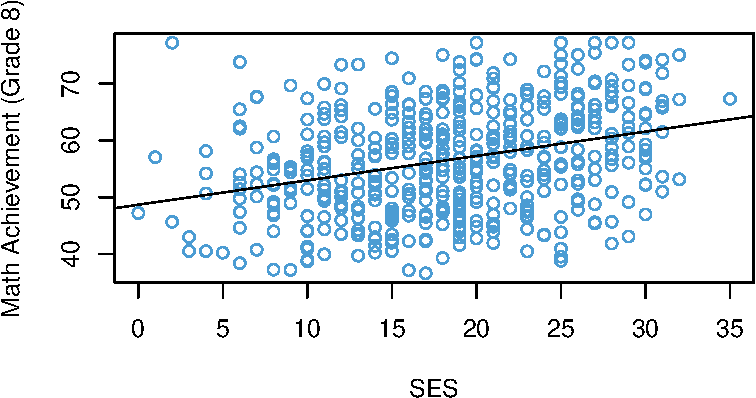
\includegraphics{ch1_review_files/figure-pdf/fig-nels-1-1.pdf}

}

\caption{\label{fig-nels-1}Math Achievement and SES (NELS88).}

\end{figure}

\bookmarksetup{startatroot}

\hypertarget{sec-chap-2}{%
\chapter{Simple Regression}\label{sec-chap-2}}

The focus of this course is linear regression with multiple predictors
(AKA \emph{multiple regression}), but we start by reviewing regression
with one predictor (AKA \emph{simple regression}).

\hypertarget{example-2}{%
\section{An example from NELS}\label{example-2}}

Figure @ref(fig:fig1) shows the relationship between Grade 8 Math
Achievement (percent correct on a math test) and Socioeconomic Status
(SES; a composite measure on a scale from 0-35). The data are a
subsample of the 1988 National Educational Longitudinal Survey (NELS;
see \url{https://nces.ed.gov/surveys/nels88/}).

\begin{Shaded}
\begin{Highlighting}[]
\CommentTok{\# Load and attach the NELS88 data}
\FunctionTok{load}\NormalTok{(}\StringTok{"NELS.RData"}\NormalTok{)}
\FunctionTok{attach}\NormalTok{(NELS)}

\CommentTok{\# Scatter plot}
\FunctionTok{plot}\NormalTok{(}\AttributeTok{x =}\NormalTok{ ses, }\AttributeTok{y =}\NormalTok{ achmat08, }\AttributeTok{col =} \StringTok{"\#4B9CD3"}\NormalTok{, }\AttributeTok{ylab =} \StringTok{"Math Achievement (Grade 8)"}\NormalTok{, }\AttributeTok{xlab =} \StringTok{"SES"}\NormalTok{)}

\CommentTok{\# Run the regression model}
\NormalTok{mod }\OtherTok{\textless{}{-}} \FunctionTok{lm}\NormalTok{(achmat08 }\SpecialCharTok{\textasciitilde{}}\NormalTok{ ses)}

\CommentTok{\# Add the regression line to the plot}
\FunctionTok{abline}\NormalTok{(mod) }
\end{Highlighting}
\end{Shaded}

\begin{figure}[H]

{\centering 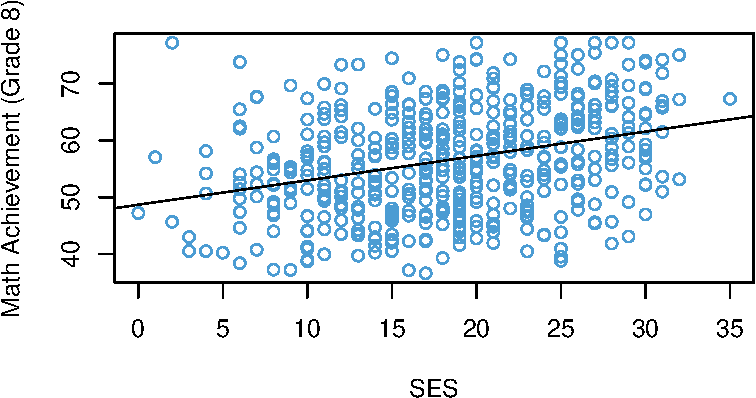
\includegraphics{ch2_simple_regression_files/figure-pdf/fig1-1.pdf}

}

\caption{Math Achievement and SES (NELS88).}

\end{figure}

The strength and direction of the linear relationship between the two
variables is summarized by their correlation (specifically, the Pearson
product moment correlation). In this sample, the correlation is

\begin{Shaded}
\begin{Highlighting}[]
\FunctionTok{options}\NormalTok{(}\AttributeTok{digits =} \DecValTok{4}\NormalTok{)}
\FunctionTok{cor}\NormalTok{(achmat08, ses)}
\end{Highlighting}
\end{Shaded}

\begin{verbatim}
[1] 0.3182
\end{verbatim}

This is a moderate, positive correlation between Math Achievement and
SES. This correlation means that eighth graders from more well-off
families (higher SES) also tended to do better in math (higher Math
Achievement).

This relationship between SES and academic achievement has been widely
documented and discussed in education research (e.g.,
\url{https://www.apa.org/pi/ses/resources/publications/education}).
\textbf{Please look over this web page and be prepared to share your
thoughts about this relationship.}

\hypertarget{regression-line-2}{%
\section{The regression line}\label{regression-line-2}}

The line in the Figure @ref(fig:fig1) can be represented mathematically
as

\[ 
\widehat Y = a + b X
(\#eq:yhat)
\]

where

\begin{itemize}
\tightlist
\item
  \(Y\) denotes Math Achievement
\item
  \(X\) denotes SES
\item
  \(a\) represents the regression intercept (the value of \(\widehat Y\)
  when \(X = 0\))
\item
  \(b\) represents the regression slope (how much \(\widehat Y\)
  increases for each unit of increase in \(X\))
\end{itemize}

Note that \(Y\) represents the values of Math Achievement in the data,
whereas \(\widehat Y\) represents the values computed from the
regression equation (i.e., the values on the regression line). The
difference \(e = Y - \widehat Y\) is called a \emph{residual}. The
residuals for a subset of the data points in Figure @ref(fig:fig1) are
shown in pink in Figure @ref(fig:fig2)

\begin{Shaded}
\begin{Highlighting}[]
\CommentTok{\# Get predicted values from regression model}
\NormalTok{yhat }\OtherTok{\textless{}{-}}\NormalTok{ mod}\SpecialCharTok{$}\NormalTok{fitted.values}

\CommentTok{\# select a subset of the data}
\FunctionTok{set.seed}\NormalTok{(}\DecValTok{10}\NormalTok{)}
\NormalTok{index }\OtherTok{\textless{}{-}} \FunctionTok{sample.int}\NormalTok{(}\DecValTok{500}\NormalTok{, }\DecValTok{30}\NormalTok{)}

\CommentTok{\# plot again}
\FunctionTok{plot}\NormalTok{(}\AttributeTok{x =}\NormalTok{ ses[index], }\AttributeTok{y =}\NormalTok{ achmat08[index], }\AttributeTok{ylab =} \StringTok{"Math Achievement (Grade 8)"}\NormalTok{, }\AttributeTok{xlab =} \StringTok{"SES"}\NormalTok{)}
\FunctionTok{abline}\NormalTok{(mod)}

\CommentTok{\# Add pink lines}
\FunctionTok{segments}\NormalTok{(}\AttributeTok{x0 =}\NormalTok{ ses[index], }\AttributeTok{y0 =}\NormalTok{ yhat[index] , }\AttributeTok{x1 =}\NormalTok{ ses[index], }\AttributeTok{y1 =}\NormalTok{ achmat08[index], }\AttributeTok{col =} \DecValTok{6}\NormalTok{, }\AttributeTok{lty =} \DecValTok{3}\NormalTok{)}

\CommentTok{\# Overwrite dots to make it look at bit better}
\FunctionTok{points}\NormalTok{(}\AttributeTok{x =}\NormalTok{ ses[index], }\AttributeTok{y =}\NormalTok{ achmat08[index], }\AttributeTok{col =} \StringTok{"\#4B9CD3"}\NormalTok{, }\AttributeTok{pch =} \DecValTok{16}\NormalTok{)}
\end{Highlighting}
\end{Shaded}

\begin{figure}[H]

{\centering 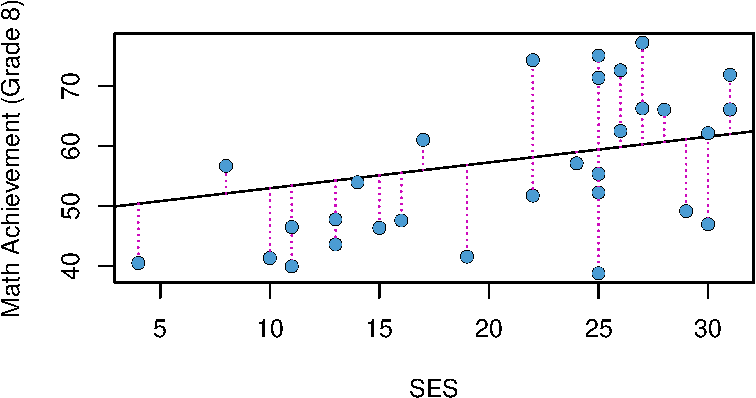
\includegraphics{ch2_simple_regression_files/figure-pdf/fig2-1.pdf}

}

\caption{Residuals for a Subsample of the Example.}

\end{figure}

Notice that \(Y = \widehat Y + e\) by definition. So, we can use either
Equation @ref(eq:yhat) or the equation below to write out a regression
model:

\begin{align} 
Y = a + bX + e.  
(\#eq:y)
\end{align}

Both equations say the same thing, but Equation @ref(eq:y) lets us talk
about the values of \(Y\) in the data, not just the predicted values.

Another way to write out the model is using the variable names (or
abbreviations) in place of the more generic ``X, Y'' notation. For
example,

\begin{align} 
\widehat {MATH} = a + b(SES). 
(\#eq:read)
\end{align}

This notation is more informative about the specific variables in the
example. But it is also more clunky and doesn't lend itself to other
mathematical expressions. For example, \(r_{XY}\) is much clearer than
\(r_{SES, MATH}\) -- in general, we want most of the text on the
``baseline'', not the subscripts or superscripts.

You should be familiar with all 3 ways of presenting regression
equations and you are free to use whatever approach you like best in
your own writing.

\hypertarget{ols-2}{%
\section{OLS}\label{ols-2}}

Intuitively, one approach to ``fitting a line to the data'' is to select
the parameters of the line (its slope and intercept) to minimize the
residuals. In ordinary least squares (OLS) regression, we minimize a
related quantity, the sum of squared residuals:

\[
\begin{align} 
SS_{\text{res}} & = \sum_{i=1}^{N} e_i^2 \\ 
& = \sum_{i=1}^{N} (Y_i - a - b X_i)^2 
\end{align} 
\]

where \(i = 1 \dots N\) indexes the respondents in the sample. OLS
regression is very widely used and is the main focus of this course,
although we will visit some other approaches in the second half of the
course.

Solving the minimization problem (setting derivatives to zero) gives the
following equations for the regression parameters:

\[ 
a = \bar Y - b \bar X \quad \quad \quad \quad b = \frac{\text{Cov}(X, Y)}{s^2_X} = r_{XY} \frac{s_Y}{s_X}
\]

(If you aren't familiar with the symbols in these equations, check out
the review materials in Section @ref(review-2) for a refresher.)

For the NELS example, the regression intercept and slope are,
respectively:

\begin{Shaded}
\begin{Highlighting}[]
\FunctionTok{coef}\NormalTok{(mod)}
\end{Highlighting}
\end{Shaded}

\begin{verbatim}
(Intercept)         ses 
    48.6780      0.4293 
\end{verbatim}

\textbf{Please write down an interpretation of these numbers in terms of
the line in Figure} @ref(fig:fig1)\textbf{, and be prepared to share
your answers in class!}

\hypertarget{correlation-and-regression}{%
\subsection{Correlation and
regression}\label{correlation-and-regression}}

Note that if \(X\) and \(Y\) are transformed to z-scores (i.e., to have
mean of zero and variance of one), then

\begin{itemize}
\tightlist
\item
  \(a = 0\)
\item
  \(b = \text{Cov}(X, Y) = r_{XY}\)
\end{itemize}

(You can check these results by plugging the value 0 for the means and
the value 1 for the variance in the equations above.)

So, regression, correlation, and covariance are all very closely related
when we consider only two variables at a time. This is why we didn't
make a big deal about simple regression in EDUC 710 -- its basically
just the same thing as correlation. But, when we get to multiple
regression (i.e., more than one \(X\) variable), we will see that
relationship between regression and correlation (and covariance) gets
more complicated.

\hypertarget{rsquared-2}{%
\section{R-squared}\label{rsquared-2}}

In the previous section we saw that the predicted value of Math
Achievement increased by .43 units (about half a percentage point) for
each unit of increase in SES. Another way to interpret this relationship
is in terms of the proportion of variance in Math Achievement that is
associated with SES -- i.e., to what extent are individual differences
in Math Achievement associated with, or explained by, individual
differences in SES?

This question is represented graphically in Figure @ref(fig:rsquared).
The horizontal line denotes the mean of Math Achievement. The difference
between the indicated student's Math Achievement score and the mean can
be divided into two parts.

\begin{itemize}
\item
  The black dashed line shows how much closer we get to the student's
  Math Achievement score (\(Y\)) by considering the predicted values
  (\(\widehat Y\)) instead of the overall mean (\(\bar Y\)). This
  represents the extent to which this student's Math Achievement is
  explained by the linear relationship with SES.
\item
  The pink dashed line is the regression residual, which was introduced
  in Section @ref(regression-line-2). This is the variation in Math
  Achievement that is ``left over'' after considering the linear
  relationship with SES.
\end{itemize}

\begin{figure}

{\centering 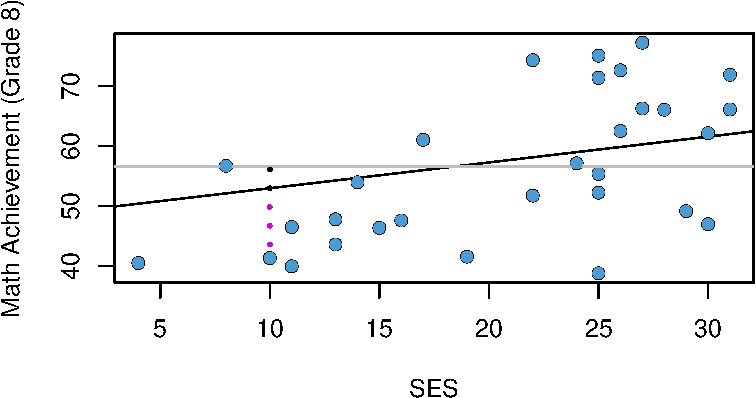
\includegraphics{ch2_simple_regression_files/figure-pdf/rsquared-1.pdf}

}

\caption{The Idea Behind R-squared.}

\end{figure}

The R-squared statistic averages the variation in Math Achievement
associated with SES (i.e., the black dashed line) relative to the total
variation in Math Achievement (i.e., black + pink) for all students in
the sample. R-squared is a widely used statistic in regression analysis,
so we will be seeing it a lot. Some authors call it the ``coefficient of
determination'' instead of R-squared.

Using all of the cases from the example (Figure @ref(fig:fig1)), the
R-squared statistic is:

\begin{Shaded}
\begin{Highlighting}[]
\FunctionTok{options}\NormalTok{(}\AttributeTok{digits =} \DecValTok{5}\NormalTok{)}
\FunctionTok{summary}\NormalTok{(mod)}\SpecialCharTok{$}\NormalTok{r.squared}
\end{Highlighting}
\end{Shaded}

\begin{verbatim}
[1] 0.10128
\end{verbatim}

\textbf{Please write down an interpretation of this number and be
prepared to share your answer in class.}

\hypertarget{derivation}{%
\subsection{Derivation*}\label{derivation}}

To derive the R-squared statistic we work the numerator of the variance,
which is called the total sum of squares.

\[SS_{\text{total}} = \sum_{i = 1}^N (Y_i - \bar Y)^2. \]

It can be re-written using the predicted values \(\widehat Y\):

\[SS_{\text{total}} = \sum_{i = 1}^N [(Y_i - \widehat Y_i) + (\widehat Y_i - \bar Y)]^2. \]

The right hand side can be reduced to two other sums of squares using
the rules of summation algebra (see the review in Section
@ref(review-2)):

\begin{align} 
SS_{\text{total}} & = \sum_{i = 1}^N (Y_i - \widehat Y_i)^2 + \sum_{i = 1}^N (\widehat Y_i - \bar Y)^2 \\
\end{align}

The first part is just \(SS_\text{res}\) from Section @ref(ols-2). The
second part is called the regression sum of squares and denoted
\(SS_\text{reg}\). Using this terminology we can re-write the above
equation as

\[ SS_{\text{total}} = SS_\text{res} + SS_\text{reg} \]

The R-squared statistic is

\[R^2 = SS_{\text{reg}} / SS_{\text{total}}. \]

As discussed above, this is interpreted as the proportion of variance in
\(Y\) that is explained by its linear relationship with \(X\).

\hypertarget{population-model-2}{%
\section{The population model}\label{population-model-2}}

In the NELS example, the population of interest is U.S. eighth graders
in 1988. We want to be able to draw conclusions about that population
based on the sample of eighth graders that participated in NELS. In
order to do that, we make some statistical assumptions about the
population, which are collectively referred to as the population model.
We talk about how to check the plausibility of these assumptions in
Chapter @ref(chapter-8).

The regression population model has the following three assumptions,
which are also depicted in the diagram below. Recall that the notation
\(Y \sim N(\mu, \sigma)\) means that a variable \(Y\) has a normal
distribution with mean \(\mu\) and standard deviation \(\sigma\).

\begin{enumerate}
\def\labelenumi{\arabic{enumi}.}
\tightlist
\item
  Normality: The values of \(Y\) conditional on \(X\), denoted \(Y|X\),
  are normally distributed (the figure shows these distributions for
  three values of \(X\)):
\end{enumerate}

\[Y | X \sim  N(\mu_{Y | X} , \sigma_{Y | X}) \]

\begin{enumerate}
\def\labelenumi{\arabic{enumi}.}
\setcounter{enumi}{1}
\tightlist
\item
  Homoskedasticity: The conditional distributions have equal variances
  (also called homegeneity of variance).
\end{enumerate}

\[ \sigma_{Y| X} = \sigma \]

\begin{enumerate}
\def\labelenumi{\arabic{enumi}.}
\setcounter{enumi}{2}
\tightlist
\item
  Linearity: The means of the conditional distributions are a linear
  function of \(X\).
\end{enumerate}

\[ \mu_{Y| Χ} = a + bX \]

\begin{figure}

{\centering 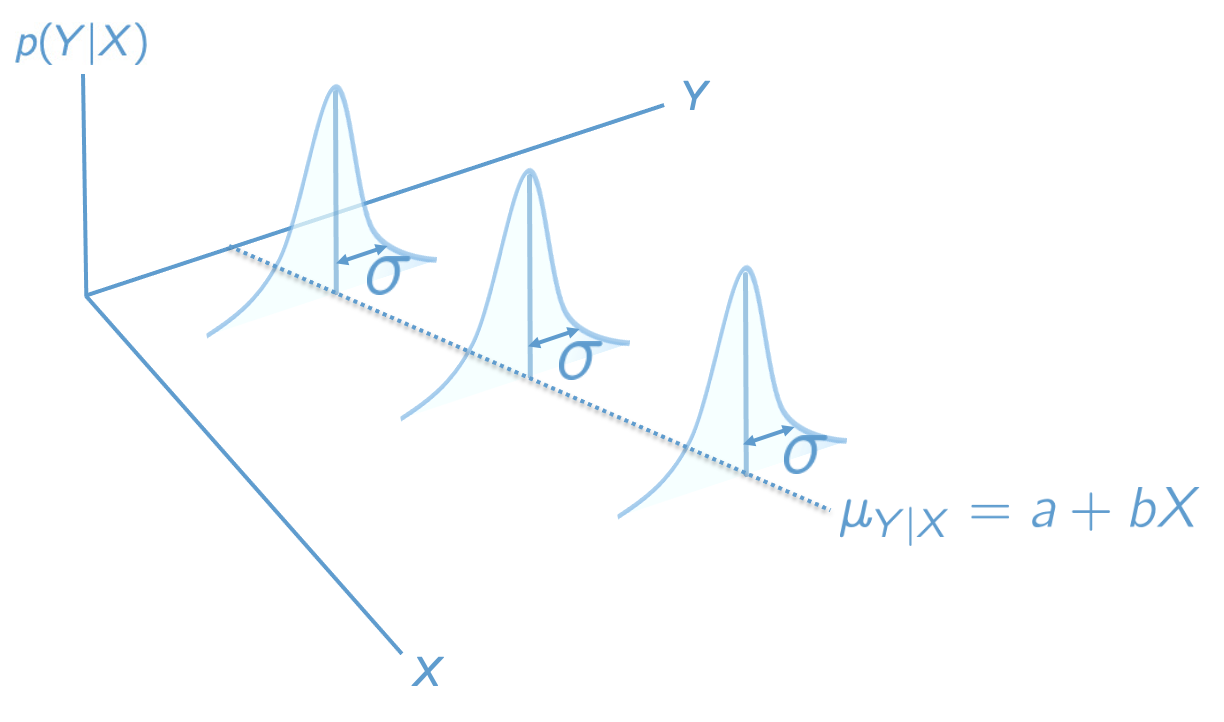
\includegraphics[width=4.08in,height=\textheight]{files/images/population_model.png}

}

\caption{The Regression Population Model.}

\end{figure}

These three assumptions are summarized by writing

\[ Y|X \sim N(a + bX, \sigma). \]

Sometimes it will be easier to state the assumptions in terms of the
population residuals, \(\epsilon = Y - \mu_{Y|X}\), which subtracts off
the regression line: \(\epsilon \sim N(0, \sigma)\).

An additional assumption is usually made about the data in the sample --
that they were obtained as a simple random sample from the population.
We will see some ways of dealing with other types of samples later on
the course, but for now we can consider this a background assumption
that applies to all of the procedures discussed in this course.

\hypertarget{notation-2}{%
\section{Clarifying notation}\label{notation-2}}

At this point we have used the mathematical symbols for regression
(e.g., \(a\), \(b\)) in two different ways:

\begin{itemize}
\tightlist
\item
  In Section @ref(regression-line-2) they denoted sample statistics.
\item
  In Section @ref(population-model-2) they denoted population
  parameters.
\end{itemize}

The population versus sample notation for regression is a bit of a hot
mess, but the following conventions are widely used.

\begin{longtable}[]{@{}lcc@{}}
\toprule\noalign{}
Concept & Sample statistic & Population parameter \\
\midrule\noalign{}
\endhead
\bottomrule\noalign{}
\endlastfoot
regression line & \(\widehat Y\) & \(\mu_{Y|X}\) \\
slope & \(\widehat b\) & \(b\) \\
intercept & \(\widehat a\) & \(a\) \\
residual & \(e\) & \(\epsilon\) \\
variance explained & \(\widehat R^2\) & \(R^2\) \\
\end{longtable}

The ``hats'' always denote sample quantities, and the Greek letters (in
this table) always denote population quantities, but there is some lack
of consistency. For example, why not use \(\beta\) instead of \(b\) for
the population slope? Well, \(\beta\) is conventionally used to denote
standardized regression coefficients in the \emph{sample}, so its
already taken (more on this in the Chapter @ref(chapter-4) ).

One thing to note is that the hats are usually omitted from the
statistics \(\widehat a\), \(\widehat b\), and \(\widehat R^2\) if it is
clear from context that we are talking about the sample rather than the
population. This doesn't apply to \(\widehat Y\), because the hat is
required to distinguish the predicted values from the data points.

Another thing to note is that while \(\widehat Y\) are often called the
predicted values, \(\mu_{Y|X}\) is not usually referred to this way. It
is called the conditional mean function or the conditional expectation
function. We will introduce some other notations for \(\widehat Y\) and
\(\mu_{Y|X}\) later in the course.

\textbf{Please be prepared for a pop quiz on notation during class!}

\hypertarget{inference-for-slope-2}{%
\section{Inference for the slope}\label{inference-for-slope-2}}

When the population model is true, \(\widehat b\) is an unbiased
estimate of \(b\). We also know the standard error of \(\widehat b\),
which is equal to (cite:fox)

\[ s_{\widehat b} = \frac{s_Y}{s_X} \sqrt{\frac{1-R^2}{N-2}} . \]

Using these two results, we can compute t-tests and confidence intervals
for the regression slope in the usual way. These are summarized below.
See the review in Section @ref(review-2) for background information on
bias, standard errors, t-tests, and confidence intervals.

\hypertarget{t-tests-1}{%
\subsection{t-tests}\label{t-tests-1}}

The null hypothesis \(H_0: \widehat b = b_0\) can be tested against the
alternative \(H_A: \widehat b \neq b_0\) using the test statistic:

\[ t = \frac{\widehat b - b_0}{s_{\widehat b}} \]

which has a t-distribution on \(N-2\) degrees of freedom when the null
hypothesis is true.

The test assumes that the population model is correct. The null
hypothesis value of the parameter is usually chosen to be \(b_0 = 0\),
in which case the test is interpreted in terms of the ``statistical
significance'' of the regression slope.

\hypertarget{confidence-intervals-1}{%
\subsection{Confidence intervals}\label{confidence-intervals-1}}

For a given Type I Error rate, \(\alpha\), the corresponding
\((1-\alpha) \times 100\%\) confidence interval is

\[ b_0 = \widehat b \pm t_{\alpha/2} \times s_{\widehat b} \]

where \(t_{\alpha/2}\) denotes the \(\alpha/2\) quantile of the
\(t\)-distribution with \(N-2\) degrees of freedom.

For example, if \(\alpha\) is chosen to be \(.05\), the corresponding
\(95\%\) confidence interval uses \(t_{.025}\), or the 2.5-th percentile
of the t-distribution.

\hypertarget{the-nels-example}{%
\subsection{The NELS example}\label{the-nels-example}}

For the NELS example, the t-test of the regression slope is shown in the
second row of the table below (we cover the rest of the output in the
next few sections):

\begin{Shaded}
\begin{Highlighting}[]
\FunctionTok{summary}\NormalTok{(mod)}
\end{Highlighting}
\end{Shaded}

\begin{verbatim}

Call:
lm(formula = achmat08 ~ ses)

Residuals:
    Min      1Q  Median      3Q     Max 
-20.600  -6.552  -0.148   6.023  27.663 

Coefficients:
            Estimate Std. Error t value Pr(>|t|)    
(Intercept)  48.6780     1.1282   43.15  < 2e-16 ***
ses           0.4293     0.0573    7.49  3.1e-13 ***
---
Signif. codes:  0 '***' 0.001 '**' 0.01 '*' 0.05 '.' 0.1 ' ' 1

Residual standard error: 8.86 on 498 degrees of freedom
Multiple R-squared:  0.101, Adjusted R-squared:  0.0995 
F-statistic: 56.1 on 1 and 498 DF,  p-value: 3.13e-13
\end{verbatim}

The corresponding \(95\%\) confidence interval is

\begin{Shaded}
\begin{Highlighting}[]
\FunctionTok{confint}\NormalTok{(mod)}
\end{Highlighting}
\end{Shaded}

\begin{verbatim}
               2.5 %   97.5 %
(Intercept) 46.46146 50.89461
ses          0.31668  0.54184
\end{verbatim}

\textbf{Please write down an interpretation of the t-test and confidence
interval of the regression slope, and be prepared to share your answers
in class!}

\hypertarget{inference-for-intercept-2}{%
\section{Inference for the intercept}\label{inference-for-intercept-2}}

The situation for the regression intercept is similar to that for the
slope: the OLS estimate is unbiased and its standard error is (cite:fox)

\[ 
s_{\widehat a} = \sqrt{\frac{SS_{\text{res}}}{N-2} \left(\frac{1}{N} + \frac{\bar X^2}{(N-1)s^2_X}\right)}.
\]

The t-tests and confidence intervals are constructed in the way same as
for the slope, just by \(a\) replacing \(b\) in the notation of the
previous slide. The t-distribution also has \(N-2\) degrees of freedom
for the intercept.

It is not usually the case that the regression intercept is of interest
in simple regression. Recall that the intercept is the value of
\(\widehat Y\) when \(X = 0\). So, unless you have a hypothesis or
research question about this particular value of \(X\) (e.g., eighth
graders with \(SES = 0\)), you won't be interested in this test (even
though R always provides it).

When we get to multiple regression, we will see some examples of
regression models where the intercept is meaningful, especially when we
talk about categorical predictors in Chapter @ref(chapter-5) and
interactions in Chapter @ref(chapter-6). But, for now, we can put it on
the back burner.

\hypertarget{inference-for-rsquared-2}{%
\section{Inference for R-squared}\label{inference-for-rsquared-2}}

Inference for R-squared is quite a bit different than for the regression
parameters. As we saw in section @ref(rsquared-2), R-squared is a ratio
of two sums of squares. We know from our study of ANOVA last semester
that ratios of sums of squares are tested using an F-test, rather than a
t-test. The F-test for (the population) R-squared is summarized below.

\hypertarget{f-tests-1}{%
\subsection{F-tests}\label{f-tests-1}}

The null hypothesis \(H_0: R^2 = 0\) can be tested against the
alternative \(H_A: R^2 \neq 0\) using the test statistic:

\[ F = (N-2) \frac{\widehat R^2}{1-\widehat R^2} \]

which has a F-distribution on \(1\) and \(N – 2\) degrees of freedom
when the null is true. The test assumes that the population model is
true. Confidence intervals for R-squared are generally not reported.

The R output from Section @ref(inference-for-slope-2) is presented again
below. \textbf{Please write down an interpretation of the F-test of
R-squared and be prepared to share your answers in class!} Note that the
output uses the terminology ``multiple R-squared'' to refer to
R-squared.

\begin{Shaded}
\begin{Highlighting}[]
\FunctionTok{summary}\NormalTok{(mod)}
\end{Highlighting}
\end{Shaded}

\begin{verbatim}

Call:
lm(formula = achmat08 ~ ses)

Residuals:
    Min      1Q  Median      3Q     Max 
-20.600  -6.552  -0.148   6.023  27.663 

Coefficients:
            Estimate Std. Error t value Pr(>|t|)    
(Intercept)  48.6780     1.1282   43.15  < 2e-16 ***
ses           0.4293     0.0573    7.49  3.1e-13 ***
---
Signif. codes:  0 '***' 0.001 '**' 0.01 '*' 0.05 '.' 0.1 ' ' 1

Residual standard error: 8.86 on 498 degrees of freedom
Multiple R-squared:  0.101, Adjusted R-squared:  0.0995 
F-statistic: 56.1 on 1 and 498 DF,  p-value: 3.13e-13
\end{verbatim}

\hypertarget{power-2}{%
\section{Power analysis}\label{power-2}}

Statistical power is the probability of rejecting the null hypothesis,
when it is indeed false. Rejecting the null hypothesis when it is false
is sometimes called a ``true positive'', meaning we have correctly
inferred that a parameter of interest is not zero. Power analysis is
useful for designing studies so that the statistical power / true
positive rate is satisfactory. In practice, this comes down to having a
large enough sample size.

Power analysis in regression is very similar to power analysis for the
tests we studied last semester. There are four ingredients that go into
a power analysis:

\begin{itemize}
\tightlist
\item
  The desired Type I Error rate, \(\alpha\).
\item
  The desired level of statistical power.
\item
  The sample size, \(N\).
\item
  The effect size, which for regression is Cohen's f-squared statistic
  (AKA the signal to noise ratio):
\end{itemize}

\[ f^2 = {\frac{R^2}{1-R^2}}. \]

In principal, we can plug-in values for any three of these ingredients
and then solve for the fourth. But, as mentioned, power analysis is most
useful when we solve for \(N\) while planning a study. When solving for
\(N\) ``prospectively,'' the effect size \(f^2\) should be based on
reports of R-squared in past research. Power and \(\alpha\) are usually
chosen to be .8 and .05, respectively.

When doing secondary data analysis (as in this class) there is not much
point in solving for the sample size, since we already have the data.
Instead, we can solve for the effect size. In the NELS example we have
\(N=500\) observations. The output below reports the smallest effect
size we can detect with a power of .8 and \(\alpha = .05\). This is
sometimes called the ``minimum detectable effect size'' (MDES). Note
that the output \(u\) and \(v\) denote the degrees of freedom in the
numerator and denominator of the F-test of R-squared, respectively.

\begin{Shaded}
\begin{Highlighting}[]
\FunctionTok{library}\NormalTok{(pwr)}
\FunctionTok{pwr.f2.test}\NormalTok{(}\AttributeTok{u =} \DecValTok{1}\NormalTok{, }\AttributeTok{v =} \DecValTok{498}\NormalTok{, }\AttributeTok{sig.level =}\NormalTok{ .}\DecValTok{05}\NormalTok{, }\AttributeTok{power =}\NormalTok{ .}\DecValTok{8}\NormalTok{)}
\end{Highlighting}
\end{Shaded}

\begin{verbatim}

     Multiple regression power calculation 

              u = 1
              v = 498
             f2 = 0.015754
      sig.level = 0.05
          power = 0.8
\end{verbatim}

\textbf{What is the MDES for the NELS example? Please be prepared to
share your answer in class.}

\hypertarget{workbook-2}{%
\section{Workbook}\label{workbook-2}}

This section collects the questions asked in this chapter. We will
discuss these questions in class. If you haven't written down / thought
about the answers to these questions before class, the lesson will not
be very useful for you! So, please engage with each question by writing
down one or more answers, asking clarifying questions, posing follow up
questions, etc.

\textbf{Section} @ref(example-2)

\begin{Shaded}
\begin{Highlighting}[]
\CommentTok{\# Scatter plot}
\FunctionTok{plot}\NormalTok{(}\AttributeTok{x =}\NormalTok{ ses, }\AttributeTok{y =}\NormalTok{ achmat08, }\AttributeTok{col =} \StringTok{"\#4B9CD3"}\NormalTok{, }\AttributeTok{ylab =} \StringTok{"Math Achievement (Grade 8)"}\NormalTok{, }\AttributeTok{xlab =} \StringTok{"SES"}\NormalTok{)}

\CommentTok{\# Run the regression model}
\NormalTok{mod }\OtherTok{\textless{}{-}} \FunctionTok{lm}\NormalTok{(achmat08 }\SpecialCharTok{\textasciitilde{}}\NormalTok{ ses)}

\CommentTok{\# Add the regression line to the plot}
\FunctionTok{abline}\NormalTok{(mod) }
\end{Highlighting}
\end{Shaded}

\begin{figure}[H]

{\centering 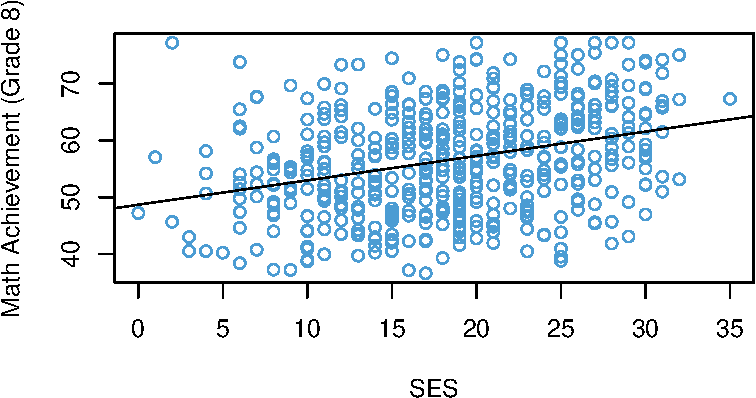
\includegraphics{ch2_simple_regression_files/figure-pdf/unnamed-chunk-8-1.pdf}

}

\caption{Math Achievement and SES (NELS88).}

\end{figure}

The strength and direction of the linear relationship between the two
variables is summarized by their correlation (specifically, the Pearson
product moment correlation). In the plot above, the correlation is

\begin{Shaded}
\begin{Highlighting}[]
\FunctionTok{options}\NormalTok{(}\AttributeTok{digits =} \DecValTok{4}\NormalTok{)}
\FunctionTok{cor}\NormalTok{(achmat08, ses)}
\end{Highlighting}
\end{Shaded}

\begin{verbatim}
[1] 0.3182
\end{verbatim}

This correlation means that eighth graders from more well-off families
(higher SES) also tended to do better in Math (higher Math Achievement).

This relationship between SES and academic achievement has been widely
documented and discussed in education research (e.g.,
\url{https://www.apa.org/pi/ses/resources/publications/education}).
Please look over this web page and be prepared to share your thoughts
about this relationship.

\textbf{Section} @ref(ols-2)

For the NELS example, the regression intercept and slope are,
respectively:

\begin{Shaded}
\begin{Highlighting}[]
\FunctionTok{coef}\NormalTok{(mod)}
\end{Highlighting}
\end{Shaded}

\begin{verbatim}
(Intercept)         ses 
    48.6780      0.4293 
\end{verbatim}

Please write down an interpretation of these numbers in terms of the
line in Figure @ref(fig:fig1), and be prepared to share your answers in
class.

\textbf{Section} @ref(rsquared-2)

Using all of the cases from the example (Figure @ref(fig:fig1)), the
R-squared statistic is:

\begin{Shaded}
\begin{Highlighting}[]
\FunctionTok{options}\NormalTok{(}\AttributeTok{digits =} \DecValTok{5}\NormalTok{)}
\FunctionTok{summary}\NormalTok{(mod)}\SpecialCharTok{$}\NormalTok{r.squared}
\end{Highlighting}
\end{Shaded}

\begin{verbatim}
[1] 0.10128
\end{verbatim}

Please write down an interpretation of this number and be prepared to
share your answer in class.

\textbf{Section} @ref(notation-2)

Please be prepared for a pop quiz on notation during class!

\begin{longtable}[]{@{}lcc@{}}
\toprule\noalign{}
Concept & Sample statistic & Population parameter \\
\midrule\noalign{}
\endhead
\bottomrule\noalign{}
\endlastfoot
regression line & & \\
slope & & \\
intercept & & \\
residual & & \\
variance explained & & \\
\end{longtable}

\textbf{Section} @ref(inference-for-slope-2)

\begin{Shaded}
\begin{Highlighting}[]
\FunctionTok{summary}\NormalTok{(mod)}
\end{Highlighting}
\end{Shaded}

\begin{verbatim}

Call:
lm(formula = achmat08 ~ ses)

Residuals:
    Min      1Q  Median      3Q     Max 
-20.600  -6.552  -0.148   6.023  27.663 

Coefficients:
            Estimate Std. Error t value Pr(>|t|)    
(Intercept)  48.6780     1.1282   43.15  < 2e-16 ***
ses           0.4293     0.0573    7.49  3.1e-13 ***
---
Signif. codes:  0 '***' 0.001 '**' 0.01 '*' 0.05 '.' 0.1 ' ' 1

Residual standard error: 8.86 on 498 degrees of freedom
Multiple R-squared:  0.101, Adjusted R-squared:  0.0995 
F-statistic: 56.1 on 1 and 498 DF,  p-value: 3.13e-13
\end{verbatim}

The corresponding \(95\%\) confidence interval is

\begin{Shaded}
\begin{Highlighting}[]
\FunctionTok{confint}\NormalTok{(mod)}
\end{Highlighting}
\end{Shaded}

\begin{verbatim}
               2.5 %   97.5 %
(Intercept) 46.46146 50.89461
ses          0.31668  0.54184
\end{verbatim}

Please write down an interpretation of the t-test and confidence
interval of the regression slope, and be prepared to share your answers
in class!

\textbf{Section} @ref(inference-for-rsquared-2)

Using the same output as above, please write down an interpretation of
the F-test of R-squared and be prepared to share your answers in class.
Note that the output uses the terminology ``multiple R-squared'' to
refer to R-squared.

\textbf{Section} @ref(power-2)

When doing secondary data analysis (as in this class) there is not much
point in solving for the sample size, since we already have the data.
Instead, we can solve for the effect size. In the NELS example we have
\(N=500\) observations. The output below reports the smallest effect
size we can detect with a power of .8 and \(\alpha = .05\). This is
sometimes called the ``minimum detectable effect size'' (MDES). Note
that the output \$u \$ and \(v\) denote the degrees of freedom in the
numerator and denominator of the F-test of R-squared, respectively.

\begin{Shaded}
\begin{Highlighting}[]
\FunctionTok{library}\NormalTok{(pwr)}
\FunctionTok{pwr.f2.test}\NormalTok{(}\AttributeTok{u =} \DecValTok{1}\NormalTok{, }\AttributeTok{v =} \DecValTok{498}\NormalTok{, }\AttributeTok{sig.level =}\NormalTok{ .}\DecValTok{05}\NormalTok{, }\AttributeTok{power =}\NormalTok{ .}\DecValTok{8}\NormalTok{)}
\end{Highlighting}
\end{Shaded}

\begin{verbatim}

     Multiple regression power calculation 

              u = 1
              v = 498
             f2 = 0.015754
      sig.level = 0.05
          power = 0.8
\end{verbatim}

What is the MDES for the NELS example? Please be prepared to share your
answer in class.

\hypertarget{exercises-2}{%
\section{Exercises}\label{exercises-2}}

These exercises collect all of the R input used in this chapter into a
single step-by-step analysis. It explains how the R input works, and
provides some additional exercises. We will go through this material in
class together, so you don't need to work on it before class (but you
can if you want.)

\hypertarget{the-lm-function}{%
\subsection{\texorpdfstring{The \texttt{lm}
function}{The lm function}}\label{the-lm-function}}

The function\texttt{lm}, short for ``linear model'', is used to estimate
linear regressions using OLS. It also provides a lot of useful output.

The main argument that the user provides to the \texttt{lm} function is
a formula. For the simple regression of Y on X, a formula has the
syntax:

\texttt{Y\ \textasciitilde{}\ X}

Here \texttt{Y} denotes the outcome variable and \texttt{X} is the
predictor variable. The tilde \texttt{\textasciitilde{}} just means
``equals'', but the equals sign \texttt{=} is already used to assign
values in R, so \texttt{\textasciitilde{}} is used in its place when
writing a formula. We will see more complicated formulas as we go
through the course. For more information on R's formula syntax, see
\texttt{help(formula)}.

Let's take a closer look using the following two variables from the NELS
data.

\begin{itemize}
\item
  \texttt{achmat08}: eighth grade math achievement (percent correct on a
  math test)
\item
  \texttt{ses}: a composite measure of socio-economic status, on a scale
  from 0-35
\end{itemize}

\begin{Shaded}
\begin{Highlighting}[]
\CommentTok{\# Load the data. Note that you can click on the .RData file and RStudio will load it}
\CommentTok{\# load("NELS.RData") \#Un{-}comment this line to run}

\CommentTok{\# Attach the data: will dicuss this in class}
\CommentTok{\# attach(NELS) \#Un{-}comment this line to run!}

\CommentTok{\# Scatter plot of math achievment against SES}
\FunctionTok{plot}\NormalTok{(}\AttributeTok{x =}\NormalTok{ ses, }\AttributeTok{y =}\NormalTok{ achmat08, }\AttributeTok{col =} \StringTok{"\#4B9CD3"}\NormalTok{)}

\CommentTok{\# Regress math achievement on SES; save output as "mod"}
\NormalTok{mod }\OtherTok{\textless{}{-}} \FunctionTok{lm}\NormalTok{(achmat08 }\SpecialCharTok{\textasciitilde{}}\NormalTok{ ses)}

\CommentTok{\# Add the regression line to the plot}
\FunctionTok{abline}\NormalTok{(mod)}
\end{Highlighting}
\end{Shaded}

\begin{figure}[H]

{\centering 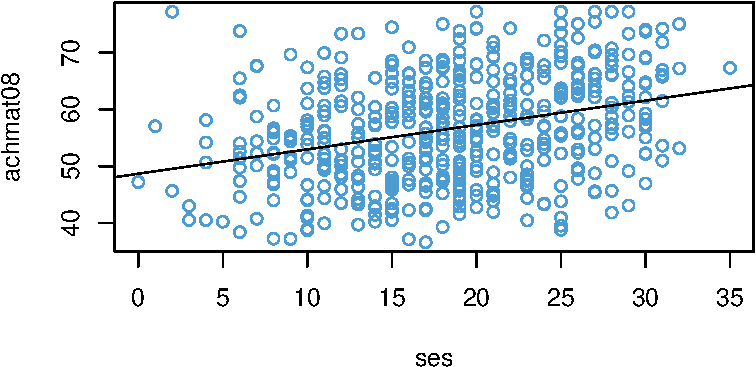
\includegraphics{ch2_simple_regression_files/figure-pdf/unnamed-chunk-15-1.pdf}

}

\end{figure}

\begin{Shaded}
\begin{Highlighting}[]
\CommentTok{\# Print out the regression coefficients}
\FunctionTok{coef}\NormalTok{(mod)}
\end{Highlighting}
\end{Shaded}

\begin{verbatim}
(Intercept)         ses 
   48.67803     0.42926 
\end{verbatim}

Let's do some quick calculations to check that the \texttt{lm} output
corresponds the formulas for the slope and intercept in Section
@ref(ols-2):

\[ a = \bar Y - b \bar X \quad \text{and} \quad b = \frac{\text{Cov}(X, Y)}{s_X^2} \]
We won't usually do these kind of ``manual'' calculations, but it is a
good way consolidate knowledge presented in the readings with the output
presented by R. It is also useful to refresh our memory about some
useful R functions and how the R language works.

\begin{Shaded}
\begin{Highlighting}[]
\CommentTok{\# Confirm that the slope from lm is equal to the covariance divided by the variance of X}
\NormalTok{cov\_xy }\OtherTok{\textless{}{-}} \FunctionTok{cov}\NormalTok{(achmat08, ses)}
\NormalTok{s\_x }\OtherTok{\textless{}{-}} \FunctionTok{var}\NormalTok{(ses)}
\NormalTok{b }\OtherTok{\textless{}{-}}\NormalTok{ cov\_xy }\SpecialCharTok{/}\NormalTok{ s\_x}
\NormalTok{b}
\end{Highlighting}
\end{Shaded}

\begin{verbatim}
[1] 0.42926
\end{verbatim}

\begin{Shaded}
\begin{Highlighting}[]
\CommentTok{\# Confirm that the y{-}intercept is obtained from the two means and the slope}
\NormalTok{xbar }\OtherTok{\textless{}{-}} \FunctionTok{mean}\NormalTok{(ses)}
\NormalTok{ybar }\OtherTok{\textless{}{-}} \FunctionTok{mean}\NormalTok{(achmat08)}

\NormalTok{a }\OtherTok{\textless{}{-}}\NormalTok{ ybar }\SpecialCharTok{{-}}\NormalTok{ b }\SpecialCharTok{*}\NormalTok{ xbar}
\NormalTok{a}
\end{Highlighting}
\end{Shaded}

\begin{verbatim}
[1] 48.678
\end{verbatim}

Let's also check our interpretation of the parameters. If the answers to
these questions are not clear, please make sure to ask in class!

\begin{itemize}
\item
  What is the predicted value of \texttt{achmat08} when \texttt{ses} is
  equal to zero?
\item
  How much does the predicted value of \texttt{achmat08} increase for
  each unit of increase in \texttt{ses}?
\end{itemize}

\hypertarget{variance-explained}{%
\subsection{Variance explained}\label{variance-explained}}

Above we found out that the regression coefficient was 0.4-ish. Another
way to describe the relationships is by considering the amount of
variation in \(Y\) that is associated with (or explained by) its
relationship with \(X\). Recall that one way to do this is via the
variance decomposition

\[ SS_{\text{total}} = SS_{\text{res}} + SS_{\text{reg}}\]

from which we can compute the proportion of variation in Y that is
associated with the regression model

\[R^2 = \frac{SS_{\text{reg}}}{SS_{\text{total}}}\]

The R-squared for the example is presented in the output below. You
should be able to provide an interpretation of this number, so if it's
not clear make sure to ask in class!

\begin{Shaded}
\begin{Highlighting}[]
\CommentTok{\# R{-}squared from the example}
\FunctionTok{summary}\NormalTok{(mod)}\SpecialCharTok{$}\NormalTok{r.squared}
\end{Highlighting}
\end{Shaded}

\begin{verbatim}
[1] 0.10128
\end{verbatim}

As above, let's compute \(R^2\) ``by hand'' for our example.

\begin{Shaded}
\begin{Highlighting}[]
\CommentTok{\# Compute the sums of squares}
\NormalTok{ybar }\OtherTok{\textless{}{-}} \FunctionTok{mean}\NormalTok{(achmat08)}
\NormalTok{ss\_total }\OtherTok{\textless{}{-}} \FunctionTok{sum}\NormalTok{((achmat08 }\SpecialCharTok{{-}}\NormalTok{ ybar)}\SpecialCharTok{\^{}}\DecValTok{2}\NormalTok{)}
\NormalTok{ss\_reg }\OtherTok{\textless{}{-}} \FunctionTok{sum}\NormalTok{((yhat }\SpecialCharTok{{-}}\NormalTok{ ybar)}\SpecialCharTok{\^{}}\DecValTok{2}\NormalTok{)}
\NormalTok{ss\_res }\OtherTok{\textless{}{-}}  \FunctionTok{sum}\NormalTok{((achmat08 }\SpecialCharTok{{-}}\NormalTok{ yhat)}\SpecialCharTok{\^{}}\DecValTok{2}\NormalTok{)}

\CommentTok{\# Check that SS\_total = SS\_reg + SS\_res}
\NormalTok{ss\_total}
\end{Highlighting}
\end{Shaded}

\begin{verbatim}
[1] 43527
\end{verbatim}

\begin{Shaded}
\begin{Highlighting}[]
\NormalTok{ss\_reg }\SpecialCharTok{+}\NormalTok{ ss\_res}
\end{Highlighting}
\end{Shaded}

\begin{verbatim}
[1] 43527
\end{verbatim}

\begin{Shaded}
\begin{Highlighting}[]
\CommentTok{\# Compute R{-}squared}
\NormalTok{ss\_reg}\SpecialCharTok{/}\NormalTok{ss\_total}
\end{Highlighting}
\end{Shaded}

\begin{verbatim}
[1] 0.10128
\end{verbatim}

\begin{Shaded}
\begin{Highlighting}[]
\CommentTok{\# Check that R{-}squared is really equal to the square of the PPMC}
\FunctionTok{cor}\NormalTok{(achmat08, ses)}\SpecialCharTok{\^{}}\DecValTok{2}
\end{Highlighting}
\end{Shaded}

\begin{verbatim}
[1] 0.10128
\end{verbatim}

\hypertarget{predicted-values-and-residuals}{%
\subsection{Predicted values and
residuals}\label{predicted-values-and-residuals}}

The \texttt{lm} function also returns the residuals \(e_i\) and the
predicted values \(\widehat{Y_i}\), which we can access using the
\texttt{\$} operator. These are useful for various reasons, especially
model diagnostics which we discuss later in the course. For now, lets
just take a look at the residual vs fitted plot to illustrate the code.

\begin{Shaded}
\begin{Highlighting}[]
\NormalTok{yhat }\OtherTok{\textless{}{-}}\NormalTok{ mod}\SpecialCharTok{$}\NormalTok{fitted.values}
\NormalTok{res }\OtherTok{\textless{}{-}}\NormalTok{ mod}\SpecialCharTok{$}\NormalTok{resid}

\FunctionTok{plot}\NormalTok{(yhat, res, }\AttributeTok{col =} \StringTok{"\#4B9CD3"}\NormalTok{)}
\end{Highlighting}
\end{Shaded}

\begin{figure}[H]

{\centering 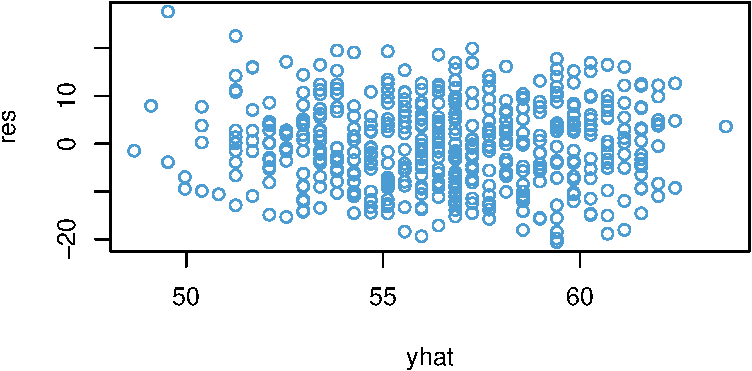
\includegraphics{ch2_simple_regression_files/figure-pdf/unnamed-chunk-19-1.pdf}

}

\end{figure}

\begin{Shaded}
\begin{Highlighting}[]
\FunctionTok{cor}\NormalTok{(yhat, res)}
\end{Highlighting}
\end{Shaded}

\begin{verbatim}
[1] -2.9515e-16
\end{verbatim}

Note that the predicted values are uncorrelated with the residuals --
this is always the case in OLS.

\hypertarget{inference}{%
\subsection{Inference}\label{inference}}

Next let's talk about statistical inference, or how we can make
conclusions about a population based on a sample from that population.

We can use the \texttt{summary} function to test the coefficients in our
model.

\begin{Shaded}
\begin{Highlighting}[]
\FunctionTok{summary}\NormalTok{(mod)}
\end{Highlighting}
\end{Shaded}

\begin{verbatim}

Call:
lm(formula = achmat08 ~ ses)

Residuals:
    Min      1Q  Median      3Q     Max 
-20.600  -6.552  -0.148   6.023  27.663 

Coefficients:
            Estimate Std. Error t value Pr(>|t|)    
(Intercept)  48.6780     1.1282   43.15  < 2e-16 ***
ses           0.4293     0.0573    7.49  3.1e-13 ***
---
Signif. codes:  0 '***' 0.001 '**' 0.01 '*' 0.05 '.' 0.1 ' ' 1

Residual standard error: 8.86 on 498 degrees of freedom
Multiple R-squared:  0.101, Adjusted R-squared:  0.0995 
F-statistic: 56.1 on 1 and 498 DF,  p-value: 3.13e-13
\end{verbatim}

In the table, the t-test and p-values are for the null hypothesis that
the corresponding coefficient is zero in the population. We can see that
the intercept and slope are both significantly different from zero at
the .05 level. However, the test of the intercept is not very meaningful
(why?).

The text below the table summarizes the output for R-squared, including
its F-test, it's degrees of freedom, and the p-value. (We will talk
about adjusted R-square in Chapter 4)

We can also use the \texttt{confint} function to obtain confidence
intervals for the regression coefficients. Use \texttt{help} to find out
more about the \texttt{confint} function.

\begin{Shaded}
\begin{Highlighting}[]
\FunctionTok{confint}\NormalTok{(mod)}
\end{Highlighting}
\end{Shaded}

\begin{verbatim}
               2.5 %   97.5 %
(Intercept) 46.46146 50.89461
ses          0.31668  0.54184
\end{verbatim}

Be sure to remember the correct interpretation of confidence intervals:
\emph{there is a 95\% chance that the interval includes the true
parameter value} (not: there is a 95\% chance that the parameter falls
in the interval). For example, there is a 95\% chance that the interval
{[}.31, .54{]} includes the true regression coefficient for SES.

\hypertarget{power-analysis}{%
\subsection{Power analysis}\label{power-analysis}}

Power analyses should ideally be done before the data are collected.
Since this class will work with secondary data analyses, most of our
analyses will be retrospective. But don't let this mislead you about the
importance of statistical power -- you should always do a power analysis
before collecting data!!

To do a power analsyis in R, we can install and load the \texttt{pwr}
package. If you haven't installed an R package before, it's pretty
straight forward -- but just ask the instructor or a fellow student if
you run into any issues.

\begin{Shaded}
\begin{Highlighting}[]
\CommentTok{\# Install the package }
\FunctionTok{install.packages}\NormalTok{(}\StringTok{"pwr"}\NormalTok{)}
\end{Highlighting}
\end{Shaded}

\begin{Shaded}
\begin{Highlighting}[]
\CommentTok{\# Load the package by using the library command}
\FunctionTok{library}\NormalTok{(}\StringTok{"pwr"}\NormalTok{)}
\end{Highlighting}
\end{Shaded}

\begin{Shaded}
\begin{Highlighting}[]
\CommentTok{\# Use the help menu to see what the package does}
\FunctionTok{help}\NormalTok{(}\StringTok{"pwr{-}package"}\NormalTok{)}
\end{Highlighting}
\end{Shaded}

To do a power analysis for linear regression, it is common to use
Cohen's \(f^2\) as the effect size:

\[f^2 = \frac{R^2}{1-R^2}.\]

Recall that \(R^2\) is the proportion of variance in \(Y\) explained by
the model, and so \(1 - R^2\) is the proportion of variance not
explained by the model. Thus, \(f^2\) can be interpreted as a signal to
noise ratio.

In addition to the effect size, we need to know the degrees of freedom
for the F-test of R-square. The \texttt{pwr} functions use the following
notation:

\begin{itemize}
\tightlist
\item
  \texttt{u} is the degrees of freedom in the numerator of an F-test.
\item
  \texttt{v} is the degrees of freedom in the denominator of an F-test.
\end{itemize}

In simple regression, \texttt{u\ =\ 1} and \texttt{v\ =\ N\ -\ 2}.

As an example of (prospective) power analysis, let's find out many
observations would be required to detect an effet size of R-square = .1,
using \(\alpha = .05\) and power = .8. To find the answer, enter the
provided information into the \texttt{pwr.f2.test} function, and the
function will solve for the ``missing piece'' -- in this case
\(v = N - 2\).

\begin{Shaded}
\begin{Highlighting}[]
\CommentTok{\# Use the provided values of R2, alpha, power (and u = 1) to solve for v = N {-} 2}
\NormalTok{R2 }\OtherTok{\textless{}{-}}\NormalTok{ .}\DecValTok{1}
\NormalTok{f2 }\OtherTok{\textless{}{-}}\NormalTok{ R2}\SpecialCharTok{/}\NormalTok{(}\DecValTok{1}\SpecialCharTok{{-}}\NormalTok{R2)}
\FunctionTok{pwr.f2.test}\NormalTok{(}\AttributeTok{u =} \DecValTok{1}\NormalTok{, }\AttributeTok{f2 =}\NormalTok{ f2, }\AttributeTok{sig.level =}\NormalTok{ .}\DecValTok{05}\NormalTok{, }\AttributeTok{power =}\NormalTok{ .}\DecValTok{8}\NormalTok{)}
\end{Highlighting}
\end{Shaded}

\begin{verbatim}

     Multiple regression power calculation 

              u = 1
              v = 70.611
             f2 = 0.11111
      sig.level = 0.05
          power = 0.8
\end{verbatim}

In this example we find that \(v = 70.6\). Since \(v = N - 2\), so we
know that a sample size of \(N = 72.6\) (rounded up to 73) is required
to reject the null hypothesis that \(R^2 = 0\), when the true population
value is \(R^2 = .1\), with a power of .8 and using a significance level
of .05.

\hypertarget{additional-exercises}{%
\subsection{Additional exercises}\label{additional-exercises}}

If time permits, we will address these additional exercises in class.

These exercises replace \texttt{achmat08} with

\begin{itemize}
\tightlist
\item
  \texttt{achrdg08}: eighth grade Reading Achievement (percent correct
  on a reading test)
\end{itemize}

Please answer the following questions using R.

\begin{itemize}
\item
  Plot \texttt{achrdg08} against \texttt{ses}. Is there any evidence of
  nonlinearity in the relationship?
\item
  What is the correlation between \texttt{achrdg08} and \texttt{ses}?
  How does it compare to the correlation with Math and SES?
\item
  How much variation in Reading is explained by SES? Is this more or
  less than for Math? Is the proportion of variance explained
  significant at the .05 level?
\item
  How much do predicted Reading scores increase for a one unit of
  increase in SES? Is this a statistically significant at the .05 level?
\item
  What are your overall conclusions about the relationship between
  Academic Achievement and SES in the NELS data?
\end{itemize}



\end{document}
